%%%%%%%%%%%%%%%%%%%%%%% file template.tex %%%%%%%%%%%%%%%%%%%%%%%%%
%
% This is a general template file for the LaTeX package SVJour3
% for Springer journals.          Springer Heidelberg 2010/09/16
%
% Copy it to a new file with a new name and use it as the basis
% for your article. Delete % signs as needed.
%
% This template includes a few options for different layouts and
% content for various journals. Please consult a previous issue of
% your journal as needed.
%
%%%%%%%%%%%%%%%%%%%%%%%%%%%%%%%%%%%%%%%%%%%%%%%%%%%%%%%%%%%%%%%%%%%
%
% First comes an example EPS file -- just ignore it and
% proceed on the \documentclass line
% your LaTeX will extract the file if required
\begin{filecontents*}{example.eps}
%!PS-Adobe-3.0 EPSF-3.0
%%BoundingBox: 19 19 221 221
%%CreationDate: Mon Sep 29 1997
%%Creator: programmed by hand (JK)
%%EndComments
gsave
newpath
  20 20 moveto
  20 220 lineto
  220 220 lineto
  220 20 lineto
closepath
2 setlinewidth
gsave
  .4 setgray fill
grestore
stroke
grestore
\end{filecontents*}
%
\RequirePackage{fix-cm}
%
\documentclass{svjour3}                     % onecolumn (standard format)
%\documentclass[smallcondensed]{svjour3}     % onecolumn (ditto)
%\documentclass[smallextended]{svjour3}       % onecolumn (second format)
%\documentclass[twocolumn]{svjour3}          % twocolumn
%
\smartqed  % flush right qed marks, e.g. at end of proof
%

% \usepackage{mathptmx}      % use Times fonts if available on your TeX system
%
% insert here the call for the packages your document requires
%\usepackage{latexsym}
% etc.
\usepackage{graphicx}
%
\usepackage{amsfonts}
\usepackage{amsmath}
\usepackage{amssymb}
\usepackage{color} % for ps_tex inclusions

% please place your own definitions here and don't use \def but
% \newcommand{}{}

\newcommand{\dataset}{{\cal D}}
\newcommand{\fracpartial}[2]{\frac{\partial #1}{\partial  #2}}

\newcommand{\I}{\mathbf I}
\newcommand{\LL}{\mathcal L}
\newcommand{\bsp}{\boldsymbol p}
\newcommand{\bss}{\boldsymbol s}
\newcommand{\BSS}{\boldsymbol S}
\newcommand{\bsx}{\boldsymbol x}
\newcommand{\BSX}{\boldsymbol X}
\newcommand{\bsy}{\boldsymbol y}
\newcommand{\BSY}{\boldsymbol Y}
\newcommand{\bbss}{\boldsymbol{\bar{s}}}
\newcommand{\BBSS}{\boldsymbol{\bar{S}}}
\newcommand{\bbsx}{\boldsymbol{\bar{x}}}
\newcommand{\BBSX}{\boldsymbol{\bar{X}}}
\newcommand{\bbsy}{\boldsymbol{\bar{y}}}
\newcommand{\BBSY}{\boldsymbol{\bar{Y}}}
\newcommand{\bslambda}{\boldsymbol \lambda}
\newcommand{\bsmu}{\boldsymbol \mu}
\newcommand{\bspi}{\boldsymbol \pi}
\newcommand{\bstheta}{\boldsymbol \theta}
\newcommand{\BSPhi}{\boldsymbol \Phi}
\newcommand{\BSSigma}{\boldsymbol \Sigma}

\newcommand{\talpha}{\tilde \alpha}
\newcommand{\tbeta}{\tilde \beta}


\newcommand{\DD}{\ensuremath{\mathbb{D}}}
\newcommand{\NN}{\ensuremath{\mathbb{N}}}
\newcommand{\RR}{\ensuremath{\mathbb{R}}}
\newcommand{\noi}{\noindent}
\newcommand{\itb}{\item[$\bullet$]}
\newcommand{\II}{\mbox{\large 1\hskip -0,353em 1}}
\newcommand{\dps}{\displaystyle}

\newcommand{\MG}{\mathcal{G}}
\newcommand{\MH}{\mathcal{H}}
\newcommand{\MM}{\mathcal{M}}
\newcommand{\MN}{\mathcal{N}}
\newcommand{\ME}{\mathcal{E}}
\newcommand{\MO}{\mathcal{O}}
\newcommand{\MP}{\mathcal{P}}
\newcommand{\MU}{\mathcal{U}}
\newcommand{\Tree}{\mathcal{T}}
\newcommand{\MV}{\mathcal{V}}

\newcommand{\card}{\mbox{card}}
\newcommand{\pa}{\mbox{pa}}
\newcommand{\spa}{\mbox{\footnotesize{pa}}}

\newcommand{\modif}[1]{\textcolor{red}{#1}}

\newtheorem{prop}{Proposition}
\newtheorem{cor}{Corollary}

% Insert the name of "your journal" with
\journalname{Statistics and Computing}
%
\begin{document}

\title{Localizing the Latent Structure Canonical Uncertainty: 
Entropy Profiles for Hidden Markov Models}

% if too long for running head
\titlerunning{Entropy profiles for hidden Markov models}        


\author{Jean-Baptiste Durand         \and
        Yann Gu\'edon %etc.
}

%\authorrunning{Short form of author list} % if too long for running head

\institute{J.-B. Durand \at
              Univ. Grenoble Alpes, Laboratoire Jean Kuntzmann and Inria, Mistis \\
	      51 rue des Math\'{e}matiques\\
	      B.P. 53, F-38041 Grenoble cedex 9, France
              Tel.: +33 4 76 63 57 09\\
              Fax: +33 4 76 63 12 63\\
              \email{jean-baptiste.durand@imag.fr}           %  \\
%             \emph{Present address:} of F. Author  %  if needed
           \and
	   Y. Gu\'edon \at 
	       CIRAD, UMR AGAP and Inria, Virtual Plants \\
	       F-34095 Montpellier, France
	       \email{guedon@cirad.fr}
}

\date{Received: date / Accepted: date}
% The correct dates will be entered by the editor


\maketitle

\begin{abstract}This paper addresses state inference for hidden Markov models. These
models rely on unobserved states, which often have a meaningful
interpretation. This makes it necessary to develop diagnostic tools for
quantification of state uncertainty. The entropy
of the state sequence that explains an observed sequence for a given hidden
Markov chain model can be considered as the canonical measure of state sequence
uncertainty. This canonical measure of state sequence uncertainty is not
reflected by the classic multidimensional posterior state (or smoothed) probability
profiles because of the marginalization that is intrinsic 
in the computation of these posterior probabilities. 
Here, we introduce a new type of profiles that have the
following properties: (i) these profiles of conditional entropies are a
decomposition of the canonical measure of state sequence uncertainty
along the sequence and makes it possible to localise this uncertainty,
(ii) these profiles are unidimensional and thus remain easily interpretable
on tree structures. We show how to extend the smoothing algorithms for
hidden Markov chain and tree models to compute these entropy profiles
efficiently. The use of entropy profiles is illustrated by 
sequence and tree data examples.
% 150 words min, 250 words max.
% here 168 words
\keywords{Conditional Entropy \and Hidden Markov Chain Model \and Hidden
 Markov Tree Model \and Plant Structure Analysis}
% \PACS{PACS code1 \and PACS code2 \and more}
% \subclass{MSC code1 \and MSC code2 \and more}
\end{abstract}



\section{Introduction}
\label{sec:introduction}
Hidden Markov chain (HMC) models have been widely used in signal processing
and pattern recognition, for the analysis of sequences with various
types of underlying structures -- for example succession of homogeneous
zones, or noisy patterns (Ephraim \& Mehrav,
2002\nocite{ephraim2002}; Zucchini \& MacDonald,
2009\nocite{zucchini2009}). This family of models was extended to other
kinds of structured data, and particularly to tree graphs
(Crouse {\it{et al.}}, 1998\nocite{crouse1998}). 
Concerning statistical inference for hidden Markov models, we distinguish
inference for the unobserved state process from inference for model parameters
(Capp\'{e} \textit{et al.}, 2005\nocite{cappe2005}).\ Our focus here
is state inference and more precisely the uncertainty in state sequences
in the HMC case. 

State inference is particularly relevant in numerous applications where
the unobserved states have a meaningful interpretation. In such cases,
the state sequence has to be restored. The restored states may be used,
typically, in prediction, in segmentation or in denoising. For example
Durand {\it et al.} (2013\nocite{durand2013}) proposed to optimise the
consumption of printers by prediction of the future printing rate from
the sequence of printing requests. This rate is related to the
parameters of an HMC model, and an optimal timeout (time before
entering sleep mode) is derived from the restored states. Le Cadre \& Tremois
(1998\nocite{lecadre1998}) used a vector of restored states in a
dynamical system for source tracking in sonar and radar systems.
Such use of the state sequence makes assessment
of the state uncertainty a critical step of the analysis.
%particularly important. 

Not only is state restoration essential for model interpretation,
it is generally used % in classical approaches 
for model diagnostic and validation as well, for example by visualising
some functions of the states. The use of restored states in the 
above-mentioned contexts raises the issue of quantifying the state
sequence uncertainty for a given observed sequence, once an HMC model
has been estimated. Global quantification of this uncertainty is 
not sufficient for a precise diagnosis: it is also very important to locate this
uncertainty along the sequence, for instance to differentiate zones that
are non-ambiguously explained from zones that are ambiguously explained
by the estimated model. We have introduced the statistical problem of quantifying state
uncertainty in the HMC model case, but the same reasoning applies to
other families of latent structure models, including hidden semi-Markov
models and hidden Markov tree (HMT) models.

Let $\BSS=\left(S_{t}\right)_{t=0,1,\ldots}$ denote the finite state
process and $J$ the number of states of an HMC model. Let
$\BSX=\left(X_t\right)_{t=0,1,\ldots}$ denote its output 
(or {\it{observed}}) process,
which takes value in an arbitrary set (countable or uncountable, 
uni- or multidimensional, \ldots). To simplify notations and without loss
of generality -- since this work focuses on conditional distributions of states 
given the outputs -- we will use $P(X_t=x_t)$ as if $X_t$ was a discrete random 
variable.
% can be either univariate, multivariate, discrete or continuous. 
Methods for exploring the state sequences that explain a
given observed sequence $\BSX=\bsx$ for a known HMC model may be divided
into three categories: 
(i) enumeration of state sequences, (ii) state profiles, which are state sequences
summarised in a $J\times T$ array where $T$ is
the length of the sequence, (iii) computation of a global measure of state
sequence uncertainty. The entropy of the state sequence that explains an
observed sequence for a known HMC model was proposed as a global
measure of the state sequence uncertainty by Hernando \textit{et al}.\
(2005\nocite{hernando2005}). We assume here that this conditional
entropy $H(\BSS|\BSX=\bsx)$ is the canonical measure of state sequence uncertainty. Various
methods belonging to these three categories have been developed for
different families of hidden Markovian models, including hidden Markov
chain and hidden semi-Markov chain models; see Gu\'{e}don
(2007b\nocite{guedon2007b}) and references therein. We identified some  
shortcomings of the proposed methods: 
\begin{itemize}
\item The entropy of the state sequence is not a summary of the state
profiles based on the posterior state (or smoothed) probabilities
$\left\{P(S_t=j|\BSX=\bsx)\right\}_{t=0,\ldots,T-1;j=0,\ldots,J-1}$,
because of the marginalization that 
is intrinsic in the computation of these probabilities. We illustrate
      using examples the fact that these state profiles contain
      artifacts, that introduce confusion between (i) local 
      state uncertainty due to overlap at $X_t=x_t$ of emission distributions
      for different states and (ii) mere propagation of uncertainty 
      from past states to current state $S_t$.
% wrongly suggesting strong state uncertainty in
%      positions where uncertainty is in fact far more limited.
\item Due to their multidimensional nature, state profiles are difficult to
visualise and interpret on trees except in the case of two-state models.
\end{itemize}

Our objective is to overcome these shortcomings, by proposing
profiles satisfying the following properties:
\begin{enumerate}
\renewcommand{\labelenumi}{(\alph{enumi})}
\item These profiles result from an additive decomposition of the the
 canonical measure of state sequence uncertainty along the sequence. 
\item Each term of the decomposition can be interpreted as a local
contribution to the global state sequence uncertainty, and thus
corresponds to a local state uncertainty. 
\item The profiles are unidimensional, and thus can be extended to more
general supporting structures such as directed acyclic graphs 
(DAGs), and in particular, trees. 
\end{enumerate}

In the case of a hidden first-order Markov chain model, applying the chain
rule (Cover and Thomas, 2006; Chapter 2\nocite{cover2006}) and the
Markovian property, the global state sequence
entropy can be decomposed as a conditional entropy profile and thus localised
along the sequence%

\begin{eqnarray}
H(\mathbf{S}|\mathbf{X}=\mathbf{x}) &=H(S_0%
|\mathbf{X}=\mathbf{x}) +\overset{T-1}{\underset{t=1}{\sum}}H(
S_{t}|S_{t-1},\ldots,S_0,\mathbf{X}=\mathbf{x}) \nonumber \\
& =H(S_0|\mathbf{X}=\mathbf{x})
+\overset{T-1}{\underset{t=1}{\sum}}H(S_{t}|S_{t-1},\mathbf{X}%
=\mathbf{x}) .
\label{eq:conditional_markov_sequence}
\end{eqnarray}

The conditional entropy profile $\left\{ H(S_t|S_{t-1}%
,\mathbf{X}=\mathbf{x}) \right\}_{t=0,\ldots,T-1}$ benefits from all
the properties of the entropy function: unique function
satisfying the Shannon-Khinchin axioms, interpretation of conditional
entropy as expected value of the entropies of the conditional
distributions, averaged over the conditioning random variables (Cover
and Thomas, 2006\nocite{cover2006}). 
We show that the posterior state probability profiles
$\left\{ P(S_t=j|\mathbf{X}=\mathbf{x}) \right\}
_{t=0,\ldots,T-1;j=0,\ldots,J-1}$ can be summarised as a marginal entropy
profile $\left\{ H(S_t|\mathbf{X}=\mathbf{x}) \right\}
_{t=0,\ldots,T-1}$ with $H(S_t|S_{t-1},\mathbf{X}=\mathbf{x})
\leq H(S_t|\mathbf{X}=\mathbf{x}) $ for $t=0,\ldots
,T-1$. Contrary to conditional entropy profiles (which can be referred to as
hidden Markov entropy profiles), marginal entropy profiles do not reflect the
state sequence uncertainty, as deduced from the conditional independence 
structure of the HMC model. We show using examples that marginal entropy profiles 
and consequently posterior state probability profiles give erroneous diagnostics and
should not be used for localising latent state structure uncertainty. 
It should be noted that a similar approach, based on conditional entropy profiles, 
has been proposed by Gu\'{e}don (2013\nocite{guedon2013}) for localizing 
the segmentation uncertainty along a sequence in the case 
of a multiple change-point model.

One of the outcomes of this work is to derive efficient
algorithms to compute the conditional entropy profile for HMC
models. 
This approach is extended to HMT models; in this case, the conditional entropy
profile is used in a first stage to identify zones with high 
local contributions to global uncertainty. In a second stage, 
state profiles computed by the Viterbi algorithm and its variants
(Durand \textit{et al}., 2004\nocite{durand2004}), or an adaption to
trees of the forward-backward Viterbi algorithm of Brushe {\it{et al.}}
(1998\nocite{brushe1998}), are visualised on selected paths of interest 
within the state process. This allows for identification of alternative
states at positions with ambiguous state value, and for better insight
on how the model associates the states with observed data.

The remainder of this paper is organized as follows. 
Section \ref{sec:profiles_hmc} focuses on algorithms to compute
conditional entropy profiles for HMC models. 
In Section \ref{sec:profiles_hmt}, an additive decomposition
of the global state entropy is derived for graphical hidden Markov
models indexed by DAGs. Then algorithms to compute conditional
entropy profiles are derived in the case of HMT models. 
The use of entropy profiles is illustrated in Section
\ref{sec:application} through applications to sequence and tree data.
Section \ref{sec:conclusion} consists of
concluding remarks. 

\section{Entropy profiles for hidden Markov chain models}
\label{sec:profiles_hmc}

In this section, HMC models are first defined. Then 
the classic forward-backward algorithm and the algorithm of Hernando
\textit{et al}. (2005\nocite{hernando2005}) to compute the 
entropy of the state sequence that explains an observed sequence are
presented. These algorithms form the basis of the proposed 
method to compute conditional entropy profiles (i.e., decomposition of the
state sequence entropy as the sum of local conditional entropies).

\subsection{Definition of a hidden Markov chain model}

A $J$-state HMC model can be viewed as a pair of discrete-time stochastic processes 
$(\BSS, \BSX)=\left( S_t, X_t\right)_{t=0,1,\ldots}$ where 
$\BSS$ is an unobserved Markov chain with finite state space $\left\{
0,\ldots,J-1\right\}$ and parameters:
\begin{itemize}
\item[$\bullet$] $\pi_j=P(S_0=j)$ with $\sum
_j \pi_j=1$ (initial probabilities), and
\item[$\bullet$] $p_{ij}=P(S_t=j|S_{t-1}=i)$
with $\sum_j p_{ij}=1$ (transition probabilities),
\end{itemize}
and where for any $\left( s_t, x_t\right)_{t=0,1,\ldots,T-1}$
\begin{align*}
& P(X_0=x_0,\ldots,X_{T-1}=x_{T-1} | S_0=s_0,\ldots,S_{T-1}=s_{T-1}) \\
& = \prod_{t=0}^{T-1} P(X_t=x_t | S_t=s_t).
\end{align*}
The output process $\BSX$ is related to the state
process $\BSS$ by the emission (or observation) probabilities 
\[
b_j(x)=P(X_t=x|S_t=j) \;\text{with
}
\sum\limits_x b_j(x)=1.
\]
Since the emission distributions
$(b_j)_{j=0,\ldots,J-1}$ are such that 
a given output $x$ may be observed in different 
states, the state process $\BSS$ cannot be deduced
without uncertainty from the outputs, but is observable only indirectly
through output process $\BSX$.
% To simplify the algorithm presentation, we consider a discrete
% univariate output process. Since this work focuses on conditional 
% distributions of states given the outputs, this assumption is not
% restrictive. 

% The definition of the emission probabilities expresses the assumption that
% $X_t$ is conditionally independent from
% $\{X_{t'}\}_{t' \neq t}$ and $\{S_{t'}\}_{t' \neq t}$ given $S_t$. 
In the sequel, $X_0^t=x_0^t$ is a shorthand for
$X_0=x_0,\ldots,X_t=x_t$ (this convention transposes to the state
sequence $S_0^t=s_0^t$). For a sequence of length $T$,
$X_0^{T-1}=x_0^{T-1}$ is simply denoted $\BSX=\bsx$ and
$S_0^{T-1}=s_0^{T-1}$ is denoted $\BSS=\bss$. In the derivation of
the algorithms for computing entropy profiles, we will use repeatedly the fact that if
$(S_t)_{t=0,1,\ldots}$ is a first-order Markov chain, the time-reversed process is
also a first-order Markov chain.

\subsection{Reminders: forward-backward algorithm and algorithm for computing the entropy of the state sequence that explains an observed sequence}
\label{subsec:hmc_reminder}
The forward-backward algorithm aims at computing the posterior state
(or smoothed) probabilities $L_t(j)=P(S_t=j|\BSX=\bsx)$
and can be stated as follows (Devijver,
1985\nocite{devijver1985}). 
The forward recursion is initialised at $t=0$ and for $j=0,\ldots,J-1$ as follows:
\begin{align}
F_0(j) & =P(S_0=j|X_0=x_0) \nonumber\\
& =\frac{b_j(x_0)}{N_0}\pi_j. \label{forward initial}%
\end{align}
The recursion is given, for $t=1,\ldots,T-1$ and $j=0,\ldots,J-1$, by:
\begin{align}
% {\mbox{for}} t=1,\ldots,T-1;\, {\mbox{for}} j=0,\ldots,J-1,\quad
F_t(j) & =P(S_t=j|X_0^t=x_0^t)
\nonumber\\
& =\frac{b_j(x_t)}{N_t}\sum\limits_{i=0}^{J-1}\,p_{ij}F_{t-1}(i). \label{forward recursion}%
\end{align}
\noindent The normalizing factor $N_t$ is obtained directly during the
forward recursion as follows%
\begin{align}
N_t & =P(X_t=x_t|X_0^{t-1}=x_0^{t-1}) \nonumber\\
& =\sum\limits_{j=0}^{J-1} P(S_t=j,X_t=x_t|X_0^{t-1}=x_0^{t-1}) ,\nonumber
\end{align}
with
\[
P(S_0=j,X_0=x_0) = b_j(x_0)\pi_j,
\]
and
\[
P(S_t=j,X_t=x_t|X_0^{t-1}=x_0^{t-1}) =b_j(
x_t) \sum\limits_{i=0}^{J-1}\,p_{ij}F_{t-1}(i).
\]
% for $t=1,\ldots,T-1$.

\noindent The backward recursion is initialised at $t=T-1$ and for
$j=0,\ldots,J-1$ as follows:
\begin{equation}
L_{T-1}( j) =P(S_{T-1}=j|\BSX=\bsx)
=F_{T-1}(j). \label{backward initial}%
\end{equation}
The recursion is given, for $t=T-2,\ldots,0$ and $j=0,\ldots,J-1$, by:
\begin{align}
% {\mbox{for }} t=T-2,\ldots,0;\, {\mbox{for }} j=0,\ldots,J-1, \quad
L_t( j) 
% =\frac{1}{N_{t+1}}\left\{ \sum\limits_{k=0}^{J-1} \frac{L_{t+1}(k) }{F_{t+1}(k) }b_k(
% x_{t+1}) p_{jk}\right\} F_t(j) \nonumber\\
& = P(S_t=j|\BSX=\bsx ) \nonumber \\ 
& = \left\{ \sum\limits_{k=0}^{J-1} \frac{L_{t+1}(k) }{G_{t+1}(k) }p_{jk}\right\}
F_t(j) , \label{backward recursion}%
\end{align}
where the predicted probability $G_{t+1}(k)$ is directly deduced from
the filtered probabilities $F_t( j)$ for the different
states $j$
\begin{align*}
G_{t+1}(k)  & 
% =F_{t+1}(k) N_{t+1}/b_{k}(
% x_{t+1}) \\
 =P(S_{t+1}=k|X_0^t=x_0^t) \\
& =\sum\limits_{j=0}^{J-1}\,p_{jk}F_t(j).
\end{align*}

% \noindent These recursions rely on conditional independence properties between
% hidden and observed variables in HMC models. Several recursions given
% in Section \ref{sec:profiles_hmc} rely on the following relations, due to
% the time-reversed process of $\left( S_t,X_t \right)_{t=0,1,\ldots}$ being also a
% hidden first-order Markov chain: for $t=1,\ldots,T-1$ and $i,j=0,\ldots,J-1$,
% \begin{align*}
% P(S_{t-1}=i|S_t=j,\BSX=\bsx)  & =P(
% S_{t-1}=i|S_t=j,X_0^t=x_0^t) \\
% & =P(S_{t-1}=i|S_t=j,X_0^{t-1}=x_0^{t-1}) ,\\
% P(S_0^{t-1}=s_0^{t-1}|S_t=j,\BSX=\bsx)  &
% =P(S_0^{t-1}=s_0^{t-1}|S_t=j,X_0^t=x_0^t) \\
% & =P(S_0^{t-1}=s_0^{t-1}|S_t=j,X_0^{t-1}=x_0^{t-1}) .
% \end{align*}

%
% the following relations will be used:
% for any $t=2, \ldots, T$
% \begin{itemize}
% \item[$\bullet$] $S_t$ is independent from $S_0^{t-2}$ given $S_{t-1}$
% 	   and $X_0^t$;
% \item[$\bullet$] $S_{t-1}$ is independent from $X_t$ given $S_t$
% 	   and $X_0^{t-1}$.
% \end{itemize}
% (DETAIL EQUATIONS ?)

An algorithm was proposed by Hernando \textit{et al}.\
(2005\nocite{hernando2005}) for computing 
the entropy of the state sequence that explains an observed sequence in the
case of an HMC model. This algorithm includes the classic forward
recursion given by (\ref{forward initial}) and (\ref{forward
recursion}) as a building block. It requires a forward recursion on
entropies of partial state sequences $S_0^t$. 
% (In the sequel, it is
% understood that the entropy of hidden state variables refers to their
% conditional entropies given observed values.)

\noindent This algorithm is initialised at $t=1$ and for
$j=0,\ldots,J-1$ as follows:
\begin{align}
&%{\mbox{for }} j=0,\ldots,J-1,\quad 
H(S_0|S_1=j,X_0^1=x_0^1) \nonumber\\
& \quad =-\sum\limits_{i=0}^{J-1} P(S_0=i|S_1=j,X_0^1=x_0^1) \log P(
S_0=i|S_1=j,X_0^1=x_0^1). \label{entropy forward initial}%
\end{align}
% This algorithm relies on the following forward recursion:
The recursion is given, for $t=2,\ldots,T-1$ and $j=0,\ldots,J-1$, by:
\begin{align}
& %{\mbox{for }} t=2,\ldots,T-1,\; {\mbox{for }} j=0,\ldots,J-1,\quad 
H(S_0^{t-1}|S_t=j,X_0^t=x_0^t) \nonumber \\
& =-\sum\limits_{s_0,\ldots,s_{t-1}}
P(S_0^{t-1}=s_0^{t-1}|S_t=j,X_0^t=x_0^t) \log
P(S_0^{t-1}=s_0^{t-1}|S_t=j,X_0^t=x_0^t)
\nonumber\\
& =-\sum\limits_{s_0,\ldots,s_{t-2}}
\sum\limits_{i=0}^{J-1} P(S_0^{t-2}=s_0^{t-2}|S_{t-1}=i,S_t=j,X_0^t=x_0%
^t) P(S_{t-1}=i|S_t=j,X_0^t=x_0^t) \nonumber\\
& \times\left\{ \log P(S_0^{t-2}=s_0^{t-2}|S_{t-1}=i,S_t%
=j,X_0^t=x_0^t) +\log P(S_{t-1}=i|S_t=j,X_0%
^t=x_0^t) \right\} \nonumber\\
& =-\sum\limits_{i=0}^{J-1} P(S_{t-1}=i|S_t=j,X_0^{t-1}=x_0^{t-1}) \left\{
\sum\limits_{s_0,\ldots,s_{t-2}}
P(S_0^{t-2}=s_0^{t-2}|S_{t-1}=i,X_0^{t-1}=x_0^{t-1})
\right. \nonumber\\
& \left. 
%% begin phantom
\vphantom{\sum\limits_{s_0,\ldots,s_{t-2}}
P(S_0^{t-2})}
%% end phantom
\times\log P(S_0^{t-2}=s_0^{t-2}|S_{t-1}=i,X_0%
^{t-1}=x_0^{t-1}) +\log P(S_{t-1}=i|S_t=j,X_0^t%
=x_0^t) \right\} \nonumber\\
& =\sum\limits_{i=0}^{J-1} P(S_{t-1}=i|S_t=j,X_0^{t-1}=x_0^{t-1}) \left\{ H(
S_0^{t-2}|S_{t-1}=i,X_0^{t-1}=x_0^{t-1}) \right. \nonumber\\
& \quad \left. -\log P(S_{t-1}=i|S_t=j,X_0^{t-1}=x_0^{t-1})
\right\} , \label{entropy forward recursion}%
\end{align}
with
\begin{align*}
& P(S_{t-1}=i|S_t=j,X_0^t=x_0^t) \\
& =\frac{P(S_t=j,S_{t-1}%
=i|X_0^{t-1}=x_0^{t-1}) }
{P(S_t=j|X_0^{t-1}=x_0^{t-1}) }\\
& =\frac{p_{ij}F_{t-1}(i) }{G_t(j) }.
\end{align*}

\noindent Using a similar argument as in (\ref{entropy forward recursion}),
the termination step is given by
\begin{align}
& H(S_0^{T-1}|\BSX=\bsx) \nonumber\\
%& = -\sum\limits_{s_0,\ldots,s_{T-1}}
%P(S_0^{T-1}=s_0^{T-1}|\BSX=\bsx)
%\log P(S_0^{T-1}=s_0^{T-1}|\BSX=\bsx) \nonumber \\
%& = -\sum\limits_{s_0,\ldots,s_{T-2}} \sum\limits_{j=0}^{J-1}
%P(S_0^{T-2}=s_0^{T-2}|S_{T-1}=j, \BSX=\bsx)
%P(S_{T-1}=j|\BSX=\bsx) \nonumber \\
%& \times \left\{\log P(S_0^{T-2}=s_0^{T-2}|S_{T-1}=j,
% \BSX=\bsx) + \log 
%P(S_{T-1}=j|\BSX=\bsx)\right\} \nonumber \\
& = - \sum\limits_{j=0}^{J-1} P(S_{T-1}=j | \BSX=\bsx)
\left\{ \sum\limits_{s_0,\ldots,s_{T-2}} 
P(S_0^{T-2}=s_0^{T-2}|S_{T-1}=j, \BSX=\bsx)
\right. \nonumber \\
& 
\times \left. 
%% begin phantom
\vphantom{\sum\limits_{s_0,\ldots,s_{t-2}}
P(S_0^{T-2}=s_0^{T-2}|S_{T-1}=j, \BSX=\bsx)}
%% end phantom
\log P(S_0^{T-2}=s_0^{T-2}|S_{T-1}=j,
 \BSX=\bsx) + \log 
P(S_{T-1}=j|\BSX=\bsx)\right\} \nonumber \\ 
& =\sum\limits_{j=0}^{J-1} F_{T-1}( j) \left\{ H(
 S_0^{T-2}|S_{T-1}=j,\BSX=\bsx
) -\log F_{T-1}(j) \right\}.
\label{entropy forward termination}%
\end{align}
The forward recursion, the backward recursion and the algorithm of
Hernando {\it{et al.}} (2005\nocite{hernando2005}) all have complexity 
in $\MO(J^2T)$.

\paragraph{{\underline{Remark.}}}The forward recursion (\ref{entropy
forward recursion}) can be interpreted as the chain rule
\begin{align}
& H(S_0^{t-1}|S_t=j,X_0^t=x_0^t) \nonumber \\  
& = H(
S_0^{t-2}|S_{t-1},S_t=j,X_0^t=x_0^t) +H(
S_{t-1}|S_t=j,X_0^t=x_0^t) \nonumber %\label{eq:chain_rule_sequence}
\end{align}
\noindent with
\begin{align*}
& H(S_0^{t-2}|S_{t-1},S_t=j,X_0^t=x_0^t) \\
%= H(S_0^{t-2}|S_{t-1},X_0^{t-1}=x_0^{t-1}) \\
%& =-\sum\limits_{s_0,\ldots,s_{t-1}} P(S_0^{t-1}=s_0^{t-1}|S_t=j,X_0^t=x_0^t)
%\times\log P(S_0^{t-2}=s_0^{t-2}|S_{t-1}=s_{t-1},S_t=j,X_0^t=x_0^t) \\
%& =-\sum\limits_{i=0}^{J-1} P(S_{t-1}=i|S_t=j,X_0^t=x_0^t) 
%\sum\limits_{s_0,\ldots,s_{t-2}}
%P(S_0^{t-2}=s_0^{t-2}|S_{t-1}=i,X_0^{t-1}=x_0^{t-1}) \\
%& \quad \times\log P(S_0^{t-2}=s_0^{t-2}|S_{t-1}=i,X_0^{t-1}%
%=x_0^{t-1}) \\
& = \sum\limits_{i=0}^{J-1} P(S_{t-1}=i|S_t=j,X_0^{t-1}=x_0^{t-1})
H(S_0^{t-2} |S_{t-1}=i,X_0^{t-1}=x_0^{t-1})
\end{align*}
and
\begin{align*}
& H(S_{t-1}|S_t=j,X_0^t=x_0^t) \\
& =-\sum\limits_{i=0}^{J-1} P(S_{t-1}=i|S_t=j,X_0^{t-1}=x_0^{t-1}) \log P(
S_{t-1}=i|S_t=j,X_0^{t-1}=x_0^{t-1}) .
\end{align*}

\subsection{Algorithms for computing conditional entropy profiles for hidden Markov chain models}
\label{subsec:past_entropy_profiles}
In what follows, we derive algorithms to compute conditional entropy
profiles 
$\left\{ H(S_t|S_{t-1},\BSX=\bsx)\right\}_{t=0,\ldots,T-1}$.
As a byproduct, the global state sequence entropy 
$H(\BSS | \BSX=\bsx)$ can be directly extracted.

We propose a first solution where the partial state sequence entropies
$\left\{ H(S_0^t| \BSX=\bsx)\right\}_{t=0,\ldots,T-1}$ 
are computed beforehand, and the conditional entropies are deduced
from the latter. Then, we propose an alternative solution where
the conditional entropies are computed directly. 

% The profiles of conditional entropies have the noteworthy property that
% the global state sequence entropy can be decomposed as a sum of
% entropies conditional on the past states
% \eq{eq:conditional_markov_sequence}

% \begin{eqnarray}
% H(\BSS|\BSX=\bsx) =H(S_0%
% |\BSX=\bsx) +\sum\limits_{t=1}^{T-1}
% H(S_t|S_{t-1},\BSX=\bsx).
% \end{eqnarray}
% % The above equation is a particular case of Corollary
% % \ref{cor:graph_entropy} in Section \ref{subsec:graphical_hmm} and will
% % be proved in the general case, but it can also be deduced from equation
% % \eqref{forward differencing} derived later in this section. 
% This property comes from the fact that the state sequence $\BSS$ is
% conditionally a Markov chain given $\BSX=\bsx$.

% In this way, the state sequence uncertainty can be localised along the
% observed sequence, $H(S_t|S_{t-1},\BSX=\bsx)$
% representing the local contribution at time $t$ to the state sequence
% entropy. 
For $t=0,\ldots,T-1$, we have
\begin{align}
& H(S_0^t|\BSX=\bsx) \nonumber\\
& =-\sum\limits_{s_0,\ldots,s_t}
P(S_0^t=s_0^t|\BSX=\bsx) \log P(
S_0^t=s_0^t|\BSX=\bsx) \nonumber\\
& =-\sum\limits_{j=0}^{J-1}P(S_t=j|\BSX=\bsx) \left\{ \sum\limits_{s_0%
,\ldots,s_{t-1}}
P(S_0^{t-1}=s_0^{t-1}|S_t=j,X_0^t=x_0^t) \right.
\nonumber\\
& \quad \left.
\vphantom{\sum_{s}P(s)}
\times \log P(S_0^{t-1}=s_0^{t-1}|S_t=j,X_0^t%
=x_0^t) +\log P(S_t=j|\BSX=\bsx)
\right\} \nonumber\\
& =\sum\limits_{j=0}^{J-1}L_t( j) \left\{ H(S_0^{t-1}|S_t=j,X_0^t%
=x_0^t) -\log L_t( j) \right\}.
\label{partial entropy recursion}
%& =\sum\limits_{j=0}^{J-1}L_t( j) H(S_0^{t-1}|S_t=j,X_0^t=x_0%
%^t) +H(S_t|\BSX=\bsx) . \nonumber
\end{align}

\noindent This recursion relies on the relation
\[
P(S_0^{t-1}=s_0^{t-1}|S_t=j,\BSX=\bsx) =P(S_0^{t-1}=s_0^{t-1}|S_t=j,X_0^t=x_0^t)
\]
due to the time-reversed process of $\left( S_t,X_t \right)_{t=0,1,\ldots}$ being also a hidden first-order Markov chain.

% Since $S_0^{t-1}$ is conditionally independent from
% $X_{t+1}^{T-1}$ given $S_t$ and $X_0^t$, we have 
% \[
% H(S_0^{t-1}|S_t,\BSX=\bsx) =H(
% S_0^{t-1}|S_t,X_0^t=x_0^t).
% \]
% Thus, application of the chain rule gives:
% \begin{align}
% & H(S_0^t|\BSX=\bsx)
% = H(S_0^{t-1}| S_t, \BSX=\bsx)
% + H(S_t | \BSX=\bsx) \nonumber\\
% & =\sum\limits_{j=0}^{J-1}{%
%TCIMACRO{\tsum }%
%BeginExpansion
% {\textstyle\sum}
%EndExpansion
% }L_t( j) H(S_0^{t-1}|S_t=j,X_0^t=x_0%
% ^t) +H(S_t|\BSX=\bsx) .
% \label{partial entropy recursion}%
% \end{align}

%\noindent Using a similar argument as in \eqref{eq:chain_rule_sequence}, equation 
%\eqref{partial entropy recursion} can be interpreted as the chain rule
%$$
% H(S_0^t| \BSX=\bsx ) %\nonumber \\  
% = H(S_0^{t-1}|S_t, \BSX=\bsx )
%+H(S_t|\BSX=\bsx )
%$$

In this way, the partial state sequence entropies $\left\{
H(S_0^t|\BSX=\bsx)\right\}_{t=0,\ldots,T-1}$ 
can be computed as a byproduct of the
forward-backward algorithm where the usual forward recursion
(\ref{forward recursion}) and the recursion (\ref{entropy forward recursion})
proposed by Hernando {\it{et al.}} (2005\nocite{hernando2005}) are
mixed. The conditional entropies are
then directly deduced by first-order differencing
\begin{align}
H(S_t|S_{t-1},\BSX=\bsx)  & =H(
S_t|S_0^{t-1},\BSX=\bsx) \nonumber\\
& =H(S_0^t|\BSX=\bsx) -H(S_0%
^{t-1}|\BSX=\bsx) .\label{forward differencing}%
\end{align}

As an alternative, the profile of conditional entropies 
$\left\{ H(
S_t|S_{t-1},\BSX=\bsx)\right\}_{t=0,\ldots,T-1}$ 
could also be computed directly, as%
\begin{align}
& H(S_t|S_{t-1},\BSX=\bsx) \nonumber \\
& =-\sum\limits_{i,j=0}^{J-1}
P(S_t=j,S_{t-1}=i|\BSX=\bsx) \log P(
S_t=j|S_{t-1}=i,\BSX=\bsx)
\label{eq:conditional_entropy_cmc}
\end{align}
with%
\begin{equation}
\left\lbrace
\begin{array}{ll}
P(S_t=j|S_{t-1}=i,\BSX=\bsx)  & =L_t(
j) p_{ij}F_{t-1}(i) /\left\{ G_t( j)
L_{t-1}( i) \right\} {\mbox{ and }}\\
P(S_t=j,S_{t-1}=i|\BSX=\bsx)  & =L_t(
j) p_{ij}F_{t-1}(i) /G_t(j).
\end{array}
\right.
\label{eq:posterior_prob_hmc}
\end{equation}
These latter quantities are directly extracted during the backward recursion
(\ref{backward recursion}) of the forward-backward algorithm. 

In summary, a first possibility is to compute the partial
state sequence entropies 
$\left\{ H(S_0^t|\BSX=\bsx)\right\}_{t=0,\ldots,T-1}$ 
using the usual forward and backward recursions
combined with
(\ref{entropy forward initial}),
(\ref{entropy forward recursion}) and (\ref{partial entropy recursion}),
from which the profile of conditional entropies 
$\left\{ H(S_t
|S_{t-1},\BSX=\bsx)\right\}_{t=0,\ldots,T-1}$ 
is directly deduced by first-order differencing
(\ref{forward differencing}).
A second possibility is to compute the 
profile of conditional entropies directly using
the usual forward and backward recursions 
combined with
\eqref{eq:conditional_entropy_cmc}
and to deduce global state sequence entropy by
summation.
The time complexity of both algorithms is in $\MO(J^2T)$.

The conditional entropy is bounded from above by the marginal
entropy (Cover \&Thomas, 2006, chap. 2):
\[
H(S_t|S_{t-1},\BSX=\bsx) \leq H(
S_t|\BSX=\bsx) ,
\] 
with%
\begin{align*}
H(S_t|\BSX=\bsx) & =-\sum\limits_{j=0}^{J-1}
P(S_t=j|\BSX=\bsx) \log P(S_t%
=j|\BSX=\bsx) \\ 
& =-\sum\limits_{j=0}^{J-1}L_t(j) \log L_t(j) .
\end{align*}
The difference between the marginal and the conditional entropy is
the mutual information $I(S_t; S_{t-1} | \BSX=\bsx)$ between $S_t$ and $S_{t-1}$, 
given $\BSX=\bsx$. Thus, the marginal entropy profile $\,$
$\left\{ H(S_t| \BSX = \bsx) \right\}_{t=0,\ldots,T-1}$ can be
viewed as pointwise upper bounds on the conditional entropy profile 
$\left\{H(S_t|S_{t-1},\BSX=\bsx)\right\}_{t=0,\ldots,T-1} $. 
The marginal entropy profile
can be interpreted as a summary of the classic
multidimensional posterior state probability profiles
$\left\{P(S_t=j|\BSX=\bsx)\right\}_{t=0,\ldots,T-1; j=0,\ldots,J-1}$. 
Hence, approximating the global state sequence uncertainty using
the sum of mar\-gi\-nal entropies $\sum_{t=0}^{T-1} H(S_t|\BSX=\bsx)$ would result into
the approximation error $\sum_{t=0}^{T-1} \{H(S_t|\BSX~=~\bsx) - H(S_t|S_{t-1},\BSX=\bsx) \}$. 
% can be used as a measure of the difference of 
% seen as a defect of the classic state profiles.

% \paragraph{Entropy profiles conditional on the future for hidden Markov
%   chain models.}
% The Markov property, which states that the past and the future are independent
% given the present, essentially treats the past and the future symmetrically.
% However, there is a lack of symmetry in the parameterization of a Markov
% chain, with the consequence that only the state process conditional on
% the past is often investigated. However, the state uncertainty at time
% $t$ may be better explained by the values of future states than past
% states. Consequently, in the present context of state inference, we
% chose to investigate the state process both forward and backward 
% in time. 

% This backward approach, described in detail in Appendix \ref{future entropy
% profiles}, relies on entropy profiles 
% $\left\{H(S_t|S_{t+1},\BSX=\bsx)\right\}_{t=0,\ldots, T-1}$
% conditional on the future states. The entropies conditional on
% the future states can also be interpreted as local contributions to 
% the global state sequence entropy, as
% \[
% H(\BSS|\BSX=\bsx)
% =\sum\limits_{t=0}^{T-2}
% H(S_t|S_{t+1},\BSX=\bsx) +H(
% S_{T-1}|\BSX=\bsx).
% \]
% The conditional entropies $H(S_t|S_{t+1},\BSX=\bsx)$ are associated
% with profiles of partial state sequence entropies
% $\left\{H(S_t^{T-1}|\BSX=\bsx)\right\}_{t=T-1,\ldots,0}$. As in the case
% of entropy profiles conditional on the past states, these profiles of
% conditional and of partial state sequence entropies can be deduced from
% each other, which leads to two algorithms of complexities in $\MO(J^2T)$.

\section{Entropy profiles for hidden Markov tree models}
\label{sec:profiles_hmt}

In this section, HMT models are introduced, as a
particular case of graphical hidden Markov (GHM) models. A generic
additive decomposition of state entropy in GHM models is proposed, and
its implementation is discussed in the case of HMT
models.

\subsection{Graphical hidden Markov models}
\label{subsec:graphical_hmm}
Let $\MG$ be a fixed (i.e. non-random), finite or infinite
directed acyclic graph (DAG) with vertex set $\MU$. A GHM 
model is a probabilistic model for observed random variables
$\BSX = (X_u)_{u \in \MU}$ indexed by $\MU$. The distribution of $\BSX$
depends on a hidden (i.e. unobserved) $J$-state process 
$\BSS = (S_u)_{u \in \MU}$ indexed by $\MU$.
% and $\BSS = (S_u)_{u \in \MU}$ be a $J$-state process indexed by $\MU$.
Let $\MG(\BSS)$ be the graph with vertices $\BSS$, isomorphic to
$\MG$ (so that the set of vertices of $\MG(\BSS)$ may be assimilated
with $\MU$). 
Let $\pa(u)$ denote the set of parents of $u \in \MU$. For any subset
$E$ of $\MU$, let $\BSS_E$ denote $(S_u)_{u \in E}$ (set of variables 
in $\BSS$ which index belongs to $E$).
GHM models assume that the following factorization of $P_{\BSS}$ --
associated with the local Markov property on $\MG$, see Lauritzen
(1996\nocite{lauritzen1996}) -- holds for any $\bss$:
\begin{eqnarray*}
P(\BSS=\bss) =
\prod\limits_{u \in \MU} P(S_u =s_u| \BSS_{\spa(u)} = \bss_{\spa(u)}),
\end{eqnarray*}
where $P(S_u =s_u| \BSS_{\spa(u)} = \bss_{\spa(u)})$ must be understood as 
$P(S_u =s_u)$ if $\pa(u) = \emptyset$. The local Markov property on
$\MG$ states that conditionally on $\BSS_{\spa(u)} = \bss_{\spa(u)}$,
$S_u$ does not depend on $S_v$ for every vertex $v$ such that there is
no path from $u$ to $v$ ($v$ is not a descendant of $u$).
% The states 
% $S_u$ are observed indirectly through an 
The output (or {\it{observed}}) process
$\BSX = (X_u)_{u \in \MU}$ is such that given $\BSS$,
% (also denoted by $\BBSS=\bbss$), 
the $(X_u)_{u \in \MU}$ are independent, and for any $u$, $X_u$
is independent of $(S_v)_{v \in \MU; v \neq u}$ given $S_u$. 
Moreover, it is assumed that given $S_u=j$, $X_u=x$ has probabiliy $b_j(x)$.
Process $\BSX$ is referred to as a GHM model with respect to DAG
$\MG$. 

In the particular case where $\MG$ is a rooted tree graph, $\BSX$ is
called a hidden Markov out-tree model with conditionally-independent children
states, given their parent state (or more shortly, an HMT
model). This model was introduced by Crouse {\it{et al.}}
(1998\nocite{crouse1998}) in the context of signal and image processing
using wavelet trees. The state process $\BSS$ is called a Markov tree.

The following notations will be used for a tree graph $\Tree$: for any vertex
$u$, $c\left( u\right)$ denotes the set of children of $u$ and
$\rho\left( u\right) $ denotes its parent. Let $\Tree_u$ denote the
subtree rooted at vertex $u$, $\BBSX_{u}=\bbsx_{u}$ denote the 
observed subtree rooted at $u$, $\BBSX_{c\left(  u\right)
}=\bbsx_{c\left(u\right)  }$ 
denote the collection of observed subtrees rooted at children of vertex $u$
(that is, subtree $\bbsx_{u}$ except its root $x_{u}$),
$\BBSX_{v\backslash u}=\bbsx_{v\backslash u}$ the subtree
$\bbsx_v$ except the subtree $\bbsx_u$ (assuming that
$\bbsx_u$ is a proper subtree of $\bbsx_{v}$), and finally
$\BBSX_{b(u)}=\bbsx_{b(u)}$ the family of brother
subtrees $(\BBSX_v)_{v \in c(\rho(u)); v \neq u}$ of $u$ (assuming that $u$
is not the root vertex).
Let $\MV$ be a subtree of $\Tree$ and let $\BBSX_\MV=\bbsx_\MV$ denote
the process $(X_u)_{u \in \MV}$, i.e., the observed subtree indexed by
$\MV$. 
This notation
transposes to the state process with for instance 
$\BBSS_{u}=\bbss_{u}$, the state subtree rooted at vertex $u$.
In the sequel, we will use the notation $\MU=\{0,\ldots,n-1\}$ to denote
the vertex set of a tree with size $n$, and the root vertex will be
$u=0$. Thus, the entire observed tree can be denoted by $\BBSX_0=\bbsx_0$,
although the shorter notation $\BSX=\bsx$ will be used hereafter. These
notations are illustrated in Figure~\ref{fig:notations} (from Durand
{\it et al.}, 2004\nocite{durand2004}).

\begin{figure}[hbtp]
\begin{center}
%\hline
\begin{picture}(0,0)%
\includegraphics{ud_gen_tree_jmlr.pstex}%
\end{picture}%
\setlength{\unitlength}{1579sp}%
%
\begingroup\makeatletter\ifx\SetFigFont\undefined%
\gdef\SetFigFont#1#2#3#4#5{%
  \reset@font\fontsize{#1}{#2pt}%
  \fontfamily{#3}\fontseries{#4}\fontshape{#5}%
  \selectfont}%
\fi\endgroup%
\begin{picture}(6809,8797)(579,-9007)
\put(5616,-3356){\makebox(0,0)[lb]{\smash{\SetFigFont{9}{10.8}{\rmdefault}{\mddefault}{\updefault}{\color[rgb]{0,0,0}$X_v$}%
}}}
\put(5381,-316){\makebox(0,0)[lb]{\smash{\SetFigFont{9}{10.8}{\rmdefault}{\mddefault}{\updefault}{\color[rgb]{0,0,0}$X_0$}%
}}}
\put(1736,-3976){\makebox(0,0)[lb]{\smash{\SetFigFont{7}{8.4}{\rmdefault}{\mddefault}{\updefault}{\color[rgb]{0,0,0}${\boldsymbol{\bar X}}_{v \setminus u}$}%
}}}
\put(6901,-5791){\makebox(0,0)[lb]{\smash{\SetFigFont{9}{10.8}{\rmdefault}{\mddefault}{\updefault}{\color[rgb]{0,0,0}$X_u$}%
}}}
\put(5401,-8836){\makebox(0,0)[lb]{\smash{\SetFigFont{7}{8.4}{\rmdefault}{\mddefault}{\updefault}{\color[rgb]{0,0,0}${\boldsymbol{\bar X}}_{{\boldsymbol c}(u)}$}%
}}}
\put(5476,-4261){\makebox(0,0)[lb]{\smash{\SetFigFont{9}{10.8}{\rmdefault}{\mddefault}{\updefault}{\color[rgb]{0,0,0}$X_{\rho(u)}$}%
}}}
\put(2726,-8386){\makebox(0,0)[lb]{\smash{\SetFigFont{7}{8.4}{\rmdefault}{\mddefault}{\updefault}{\color[rgb]{0,0,0}${\boldsymbol{\bar X}}_u$}%
}}}
\put(254,-5774){\makebox(0,0)[lb]{\smash{{\SetFigFont{7}{8.4}{\rmdefault}{\mddefault}{\updefault}{\color[rgb]{0,0,0}${\boldsymbol{\bar X}}_{b(u)}$}%
}}}}
\end{picture}
\caption[Markov tree]
{\label{fig:notations}{\textit{The notations used for indexing
subtrees of observed tree $\BSX=\BBSX_0$. These notations
transpose to the state tree $\BSS=\BBSS_0$.}}}
%\hline
\end{center}
\end{figure}

Let $\Tree$ be a fixed tree with vertex set $\MU$.
A $J$-state HMT model $(\BSS, \BSX) = (S_u, X_u)_{u \in \MU}$ on $\Tree$ 
is defined by the following parameters: 
\begin{itemize}
\item[$\bullet$] $\pi_j=P\left(
S_0=j\right)  $ with $\sum_j\pi_j=1$ (initial probabilities for the root vertex),
\item[$\bullet$] $p_{jk}=P\left(  S_{u}=k|S_{\rho\left(
u\right)  }=j\right)  $ with $\sum_{k}p_{jk}=1$ (transition probabilities),
\end{itemize}
and by the emission distributions defined as in HMC models by 
$b_j(x)=P(X_u = x | S_u = j)$.

In GHM models, the state process is conditionally Markovian in the
following sense:
\begin{prop}
Let $(\BSS, \BSX)$ be a GHM model with respect to DAG $\MG$. Then for
any $\bsx$, the conditional distribution of 
$\BSS$ given $\BSX=\bsx$ satisfies the Markov property on $\MG$ and
for any $\bss$, 
\[
P(\BSS=\bss | \BSX=\bsx) = 
\prod\limits_u P(S_u =s_u| \BSS_{\spa(u)} = \bss_{\spa(u)}, \BSX=\bsx),
\]
where $P(S_u =s_u| \BSS_{\spa(u)} = \bss_{\spa(u)}, \BSX=\bsx)$ denotes
$P(S_u =s_u| \BSX=\bsx)$ if $pa(u) = \emptyset$.
\label{prop:conditional_markov}
\end{prop}
\begin{proof}
To prove this proposition, we consider a potential realization $(\bss,
\bsx)$ of process $(\BSS, \BSX)$. We introduce the following definitions
and notations: for $u \in \MU$, $An(u)$ denotes the set of ancestors of
 $u$ in $\MG$; for $A \subset U$, $An(A)=\{An(u)\}_{u \in A}$ 
and ${\bar An}(A)=An(A) \cup A$. Let $\BSS_A=\bss_A$ denote the state
process indexed by the graph induced by $A$.
By conditional independence of the $(X_u)_{u \in \MU}$ given
$\BSS$, the process $(\BSS, \BSX)$ follows the Markov property on
the DAG $\MG(\BSS, \BSX)$ obtained from $\MG(\BSS)$ by addition of the set
of vertices $\{X_u | u \in \MU\}$ and the set of arcs $\{(S_u, X_u) | u
\in \MU \}$. 

It is proved by induction on subgraphs $A$ of $\MG$ that 
if ${\bar An}(A)=A$, then 
\begin{eqnarray}
P(\BSS_A=\bss_A | \BSX=\bsx) = 
\prod\limits_{v \in A}
P(S_v =s_v| \BSS_{\spa(v)} = \bss_{\spa(v)}, \BSX=\bsx).
\label{eq:induction}
\end{eqnarray}
Since the joint distribution of state vertices in different connected
components $(\MG_1,\ldots,\MG_C)$ of $\MG$ can be factorised as 
$\prod_c P(\BSS_{\MG_c}=\bss_{\MG_c} | \BSX=\bsx )$,
equation \eqref{eq:induction} is proved separately for each connected
component. 

It is easily seen that if $u$ is a source vertex of $\MG$ (vertex
without parents), both the right-hand 
and the left-hand sides of equation \eqref{eq:induction} are equal to 
$P(S_u = s_u|\BSX=\bsx )$. To prove the induction step, we consider a
vertex $u \notin A$ such that $\pa(u) \subset A$. If such vertex does
not exist, $A$ is a connected component of $\MG$, which terminates the
induction. 

Otherwise, let $A'$ denote $A \cup \{u\}$. Then ${\bar An}(A')=A'$ and
\begin{align*}
P(\BSS_{A'}=\bss_{A'} | \BSX=\bsx)
= & P(S_u = s_u | \BSS_{\spa(u)}=\bss_{\spa(u)}, 
\BSS_{A \backslash \spa(u)}=\bss_{A \backslash \spa(u)}, \BSX=\bsx) \\
 \quad & \times P(\BSS_{\spa(u)}=\bss_{\spa(u)}, 
\BSS_{A \backslash \spa(u)}=\bss_{A \backslash \spa(u)}
| \BSX=\bsx) \nonumber \\
= &  P(S_u = s_u | \BSS_{\spa(u)}=\bss_{\spa(u)}, \BSX=\bsx)
 P(\BSS_A=\bss_A | \BSX=\bsx)
\end{align*}
since the Markov property on $\MG(\BSS, \BSX)$ implies conditional
independence of $S_u$ and $\BSS_{A \backslash \spa(u)}$ given
$S_{\spa(u)}$ and $\BSX$. 

The proof is completed by application of induction equation
\eqref{eq:induction}. $\blacksquare$
\end{proof}

%From application of the chain rule
%(Cover \& Thomas, 2006, chap. 2\nocite{cover2006}) and Proposition
%\ref{prop:conditional_markov}, t
%
The following corollary is derived from Proposition
\ref{prop:conditional_markov}:
\begin{cor}
Let $(\BSS, \BSX)$ be a GHM model with respect to DAG $\MG$. Then 
for any $\bsx$,
\[
H(\BSS | \BSX=\bsx) = 
\sum\limits_u H(S_u | \BSS_{\spa(u)}, \BSX=\bsx),
\]
where $H(S_u | \BSS_{\spa(u)}, \BSX=\bsx)$ denotes
$H(S_u | \BSX=\bsx)$ if $\pa(u) = \emptyset$.
\label{cor:graph_entropy}
\end{cor}
\begin{proof}
This corollary results from 
\begin{align*}
H(\BSS | \BSX=\bsx) = & E\left[\log P(\BSS | \BSX=\bsx)|
  \BSX=\bsx\right] \\
= & \sum\limits_u E\left[\log P(S_u | \BSS_{\spa(u)}, \BSX=\bsx)|
  \BSX=\bsx\right] \\
= & \sum\limits_u H(S_u | \BSS_{\spa(u)}, \BSX=\bsx)
.\blacksquare
\end{align*}
\end{proof}

This result extends equation \eqref{eq:conditional_markov_sequence} for
HMC models to hidden Markov models indexed by DAGs.

It follows from Corollary \ref{cor:graph_entropy} that the global
entropy of the state process can be decomposed as a sum of conditional
entropies, where each term is the local contribution of state $S_u$ at
vertex $u$, and corresponds to the conditional entropy of this state
given the parents' states (or equivalently, given the non-descendant
states, from the Markov property on $\MG(\BSS, \BSX)$). In practical
applications of GHM models, the unidimensional profiles 
$\left\{H(S_u | \BSS_{\spa(u)}, \BSX=\bsx)\right\}_{u \in \MU}$ are
computed in a first stage, to identify vertices in $\MU$ associated 
with high local contributions to global uncertainty.
% uncertainty is locally high. 
In a second stage, the Viterbi algorithm
and its variants are used to investigate alternative state
restorations. 

The remainder of this Section focuses on the derivation of algorithms to
compute entropy profiles efficiently in HMT models.

\subsection{Reminder: upward-downward algorithm}
\label{subsec:hmt_reminder}
The upward-downward algorithm aims at computing the posterior state
probabilities $\xi_{u}(j)=P(S_{u}=j|\BSX=\bsx)$ and can be stated as
follows (Durand {\it{et al.}}, 2004\nocite{durand2004}). It consists in
three recursions, which all have complexities in $\MO(J^2n)$.

This algorithm requires preliminary computation of the state marginal
probabilities $P(S_u=j)$, computed by a recursion such that
every vertex must be visited after its parent vertex (referred to
as {\it{downward recursion}}). This
recursion is initialised at the root vertex $u=0$ and for
$j=0,\ldots,J-1$ as follows:
\[
% j=0,\ldots,J-1,\quad 
P(S_0=j) = \pi_j.
\]
The recursion is given, for vertices $u \neq 0$ taken downwards and
for $j=0,\ldots,J-1$, by:
\[
P(S_u=j) = \sum\limits_{i=0}^{J-1} p_{ij} P(S_{\rho(u)}=i).
\]
In the {\it{upward recursion}},every vertex must be visited 
after its children vertices. It is initialised for each leaf as follows.
For $j=0,\ldots,J-1$,
\begin{align*}
% \forall j=0,\ldots,J-1,\quad 
\beta_u(j) = & P(S_u = j | X_u = x_u)\\
 = &   \frac{
b_j(x_u) P(S_u = j)}
{N_u}.
\end{align*}
The recursion is given, for internal vertices $u$ taken upwards and
for $j=0,\ldots,J-1$, by:
\begin{align*}
% & \forall j=0,\ldots,J-1,\quad 
\beta_{\rho(u),u}(j)  =  & \frac{
P({\boldsymbol{\bar X}}_u = {\boldsymbol{\bar x}}_u | S_{\rho(u)} = j)}
{P({\boldsymbol{\bar X}}_u = {\boldsymbol{\bar x}}_u)} \\
 = & \sum\limits_{k=0}^{J-1} \frac{\beta_u(k) p_{jk}}{P(S_u = k)}
\end{align*}
and
\begin{align*}
% {\lefteqn{
% \forall j=0,\ldots,J-1,\quad 
\beta_u(j)  = &
P(S_u = j | {\boldsymbol{\bar X}}_u = {\boldsymbol{\bar x}}_u) \\
 = &  {\dps{\frac{\left\{
\prod\limits_{v \in {\boldsymbol c}(u)}\beta_{u,v}(j) \right\}
b_j(x_u) P(S_u = j)}
{N_u}}}. 
\end{align*}
The normalizing factor $N_u$ is obtained directly during the upward
recursion by
$$
N_u  = P(X_u = x_u) = \sum\limits_{j=0}^{J-1}  b_j(x_u) P(S_u = j)
$$
for the leaf vertices, and
\begin{eqnarray*}
% \lefteqn{
N_u  =  {\displaystyle{\frac
{P({\boldsymbol{\bar X}}_u = {\boldsymbol{\bar x}}_u)}
{\prod\limits_{v \in {\boldsymbol c}(u)}
P({\boldsymbol{\bar X}}_v = {\boldsymbol{\bar x}}_v)}}}
  =  \sum\limits_{j=0}^{J-1}\left\{
\prod\limits_{v \in {\boldsymbol c}(u)}\beta_{u,v}(j) \right\}
 b_j(x_u) P(S_u = j) \label{eq:cupnorm}
\end{eqnarray*}
for the internal vertices.

\noindent The downward recursion is initialised at the root vertex $u=0$
and for $j=0,\ldots,J-1$ as follows:
$$
% \forall j=0,\ldots,J-1,\quad 
\xi_0(j) = P(S_0 = j | \BSX=\bsx) = \beta_0(j)
$$
The recursion is given, for vertices $u \neq 0$ taken downwards and
for $j=0,\ldots,J-1$, by:
\begin{align}
% & \forall j=0,\ldots,J-1,\quad 
\xi_u(j) = & P(S_u = j | \BSX=\bsx) \nonumber \\
 =  & \frac{\beta_u(j)}{P(S_u = j)}
\sum\limits_{i=0}^{J-1} \frac{p_{ij} \xi_{\rho(u)}(i)}{\beta_{\rho(u),u}(i)}.
\label{eq:downward}
\end{align}

\subsection{Algorithms for computing conditional entropy profiles for hidden
Markov tree models}
In HMT models, the decomposition of global state tree entropy yielded
by Corollary \ref{cor:graph_entropy} writes
\begin{eqnarray}
H(\BSS | \BSX=\bsx) = 
H(S_0 | \BSX=\bsx) +
\sum\limits_{u \neq 0} H(S_u | S_{\rho(u)}, \BSX=\bsx).
\label{eq:hmt_decomposition}
\end{eqnarray}
This decomposition can be extended to the entropy of any state
subtree, as shown in Proposition~\ref{prop:subtree_entropy} in
Appendix~\ref{app:subtree}.
As a consequence of this decomposition, the canonical measure of state
tree uncertainty can 
be localised along the observed tree, $H(S_{u}|S_{\rho(u)},\BSX=\bsx)$
representing the local contribution at vertex $u$ to the global state tree
entropy. Note that this decomposition generalises to HMT models decomposition
\eqref{eq:conditional_markov_sequence} of HMC models.

We propose a first approach where conditional entropy profiles
$\{H(S_u | S_{\rho(u)}, \BSX=\bsx)\}_{u \in \MU}$ are directly computed
during the downward recursion \eqref{eq:downward}. As a byproduct, 
the global state tree entropy $H(\BSS | \BSX=\bsx)$
is obtained by summation. Then we propose a second approach based on
the direct computation of the conditional entropies of state subtrees.
The conditional entropy profiles are deduced from the latter.

\paragraph{Direct computation of conditional entropy profiles}
Firstly, for every non-root vertex $u$, 
the conditional entropy 
\begin{align}
& % H(\BBSS_u | S_{\rho(u)}, \BSX = \bsx)= 
H(S_u | S_{\rho(u)}, \BSX = \bsx) \nonumber \\
& = -\sum_{i,j} P(S_u = j, S_{\rho(u)} = i | \BSX = \bsx)
\log P(S_u = j | S_{\rho(u)} = i, \BSX = \bsx)
\label{eq:child_parent_entropy}
\end{align}
is directly extracted during the downward recursion \eqref{eq:downward},
similarly to \eqref{eq:posterior_prob_hmc} for HMC models, with 
\begin{equation}
\left\lbrace
\begin{array}{ll}
 P(S_u = j | S_{\rho(u)} = i, \BSX = \bsx) & = \beta_u(j) p_{ij}
/ \{P(S_u=j) \beta_{\rho(u),u}(i)\}  {\mbox{ and }} \\ 
P(S_u = j, S_{\rho(u)} = i | \BSX = \bsx) & = \beta_u(j) p_{ij} 
\xi_{\rho(u)}(i) / \{P(S_u=j) \beta_{\rho(u),u}(i)\}.
\end{array}
\right.
\label{eq:predict_upwd}
\end{equation}

The global state tree entropy $H(\BSS | \BSX = \bsx)$ is obtained
by summation of conditional entropies using \eqref{eq:hmt_decomposition}.
The time complexity of the algorithm is in $\MO(J^2n)$.
As in HMC models, the marginal entropy profile 
$\left\{H(S_{u} | \BSX = \bsx)\right\}_{u \in \MU}$ can be
viewed as pointwise upper bounds on the conditional entropy profile 
$\left\{H(S_{u} | S_{\rho(u)}, \right. \allowbreak\left. \BSX = \bsx)\right\}_{u \in \MU}$.

\paragraph{Computation of conditional entropies of children state
    subtrees given each state}
As an alternative, the entropies $H(\BBSS_{c(u)} | S_{u}=j, \BBSX_u=\bbsx_u)$
can be computed directly during the upward recursion given in Section
\ref{subsec:hmt_reminder}. These are similar to the entropies
$H(S_0^{t-1}|S_t=j,X_0^t=x_0^t)$, used in 
the algorithm of Hernando \textit{et al}. (2005\nocite{hernando2005}) in
HMC models. Therefore, the following algorithm can be seen as a
generalization of their approach to HMT models. 
As in the case of HMC models, the global state tree entropy
$H(\BSS|\BSX=\bsx)$ is obtained at the final step of the upward
recursion.
This approach, described
in detail in Appendix \ref{app:hmt_hernando}, relies on the
computation of the entropies $H(\BBSS_{c(u)}|S_{u}=j,\BBSX_u=\bbsx_u)$
for $u \in \MU, u \neq 0$ and for $j=0,\ldots,J-1$, using an upward 
recursion.

Partial state tree entropies $H(\BBSS_u | \BSX = \bsx)$ can be deduced
from the quantities $H(\BBSS_{c(u)}|S_{u}=j,\BBSX_u=\bbsx_u)$ in 
the downward recursion.
Finally, the conditional entropy profiles 
$H(S_{u} | S_{\rho(u)}, \BSX = \bsx)$ 
are extracted from the latter entropies. The time complexities of the
algorithms are in $\MO(J^2n)$. 

\section{Applications}
\label{sec:application}
To illustrate the practical ability of entropy profiles to provide
localised information on the latent state structure uncertainty, three
examples are considered.
\begin{enumerate}
\item The first one consists in a synthetic example of HMC model that
illustrates how to quantify the roles of emission distributions and
the Markovian structure in assessing global state sequence uncertainty.
\item The second one consists in the HMC analysis of the earthquake dataset, published by Zucchini \& MacDonald (2009\nocite{zucchini2009}).
The third one consists in the HMT analysis of the structure of pine branches, using an original dataset.
\end{enumerate}

It is shown in particular that entropy
profiles allow regions that are non-ambiguously explained by the
estimated model to be differentiated from regions that are ambiguously
explained. Their ability to provide accurate interpretation of the model
states is also emphasised.

\subsection{Synthetic example of HMC model}
A family of 2-state HMC models with known parameters is
considered. The transition probability matrix is 
\[
P = 
\left[
\begin{array}{cc}
1-\varepsilon    &  \varepsilon\\
\varepsilon      &  1-\varepsilon
\end{array}
\right]
\]
where $\varepsilon \in [0,0.5]$ is a known parameter. The initial
probabilities are $\pi_0 = \pi_1 = 0.5$, which correspond to the
stationary state distribution in the ergodic cases ($\varepsilon >
0$). The observed variables $X_t$ 
take values in $\{0, 1, 2\}$ and the emission distributions 
are defined by the following emission probability matrix (with
states in rows and observations in columns):
\[
B = 
\left[
\begin{array}{ccc}
0.5    &  0.5 & 0 \\
0      &  0.5 &  0.5
\end{array}
\right].
\]
Let $\bsx=x_0^{T-1}$ be defined as $x_t = 1$ for $t=0,\ldots,T-1$. For every
$t=0,\ldots,T-1$, the posterior state probabilities are $P(S_t = 0 | \BSX=\bsx) = P(S_t = 1 | \BSX=\bsx)
= 0.5$. Thus at every time $t$, the marginal
entropy is $\log 2$, independently of $\varepsilon$, and the sum of
marginal entropies is $T \log 2$. In contrast, the global state sequence
entropy is an increasing function of $\varepsilon$, with 
$H(\BSS | \BSX=\bsx) = \log 2$ for $\varepsilon = 0$ and $H(\BSS |
\BSX=\bsx) = T \log 2$ for $\varepsilon = 0.5$. 
In the case where $\varepsilon = 0$, every state is equal to the
initial state $S_0$ and the only uncertainty in the whole state
sequence is related to the value of $S_0$. Thus, the global state
sequence entropy is the initial state entropy $\log 2$. 
In this particular case, all the other states 
could be deduced from one single known state. The profile of entropies conditional on the next state $H(S_t | S_{t+1}, \BSX=\bsx)$ could also
be used to quantify local uncertainty (see also discussion 
in Section \ref{sec:conclusion}). This approach would place whole state
sequence uncertainty to the value of $S_{T-1}$, which is correct but 
inconsistent with the chosen parameterisation of the model.
In the case where $\varepsilon = 0.5$, $\BSS$ is a zero-order Markov
chain and the global state sequence entropy is also the sum of
marginal entropies $T \log 2$.

This interpretation and the associated quantification of state
sequence uncertainty are consistent with the conditional entropy
profiles depicted in Figure~\ref{fig:synthetic}. In contrast, 
the marginal entropy profiles only translate the fact that both states
are equally likely at every time $t$. In our case, they are
identical to the entropy profiles of a zero-order Markov
chain. 
% Consequently, except in the latter case, marginal entropy
% profiles do not allow quantification of the global state sequence
% uncertainty. 
While the conditional entropy profiles highlight
that new observations $X_t=1$ do not increase state sequence uncertainty, 
the marginal entropy profiles reflect propagation of state uncertainty
from a state $S_t$ to its neighbour states $S_{t-1}$ and $S_{t+1}$. 
As a consequence, except in the case of independent states, the value 
of marginal entropy cannot be interpreted in terms of local contributions
to global state uncertainty.
 % This results from these profiles not taking fully into
% account the Markovian structure.

\begin{figure}[!htb]
\begin{center}
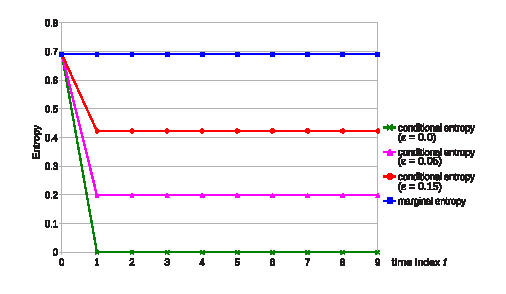
\includegraphics[scale=1.7]{synthetic_example.eps}
\caption[Synthetic example]
{\textit{Entropy profiles for 2-states HMC models with
    state transition probabilities $\varepsilon=0.0$,
    $\varepsilon=0.05$ and $\varepsilon=0.15$.}}
\label{fig:synthetic}
\end{center}
\end{figure}

\subsection{HMC analysis of earthquakes}
\label{subsec:app_hmc}

The data consists of a single sequence of annual
counts of major earthquakes (defined as of magnitude 7 and above) for
the years 1900-2000; see Figure~\ref{fig:earthquakes}. 
\begin{figure}[!htb]
%\begin{center}
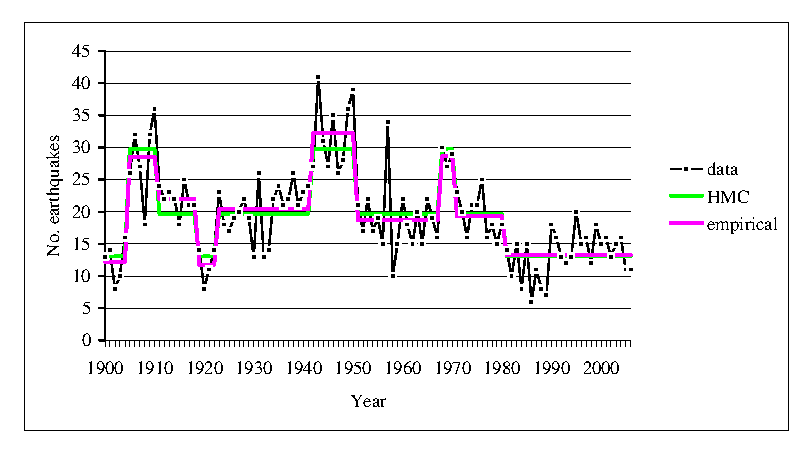
\includegraphics[scale=0.82]{earthquake1.eps}
\caption[Earthquake data]
{\textit{Earthquake data: Restored state sequence represented as step
functions, the level of the segments being either the parameter
$\widehat{\lambda}_j$\ of the Poisson emission distributions
corresponding to the restored state $j$ or the empirical mean estimated for
the segment.}}
\label{fig:earthquakes}
%\end{center}
\end{figure}

A 3-state stationary HMC model with Poisson emission
distributions was estimated
on the basis of this earthquake count
sequence using the EM algorithm -- see 
Zucchini \& MacDonald (2009\nocite{zucchini2009}). 
The estimated parameters of the Poisson emission
distributions were $\widehat{\lambda}_1=13.1$,
$\widehat{\lambda}_2=19.7$ and $\widehat{\lambda}_3=29.7$.
The restored state sequence is represented in Figure
\ref{fig:earthquakes} as step functions, the level of the segments being
either the parameter $\widehat{\lambda}_j$ of the Poisson emission
distributions corresponding to the restored state $j$ or the empirical
mean estimated for the segment. The state profiles computed by
the forward backward algorithm 
$\left\{ P(S_t=j|\BSX=\bsx)\right\}_{
t=0,\ldots,T-1;j=0,\ldots,J-1}$ 
are shown in Figure~\ref{fig:earthquakes_smoothed}. The entropy of the
state sequence that explains the observed sequence for the estimated
HMC model is bounded from above by the sum of the marginal entropies
\begin{align*}
H(\BSS|\BSX=\bsx) =\sum\limits_t
H(S_t|S_{t-1},\BSX=\bsx) & =14.9 \\
< \sum\limits_t H(S_t|\BSX=\bsx) & =19.9.
\end{align*}

\begin{figure}[!htb]
%\begin{center}
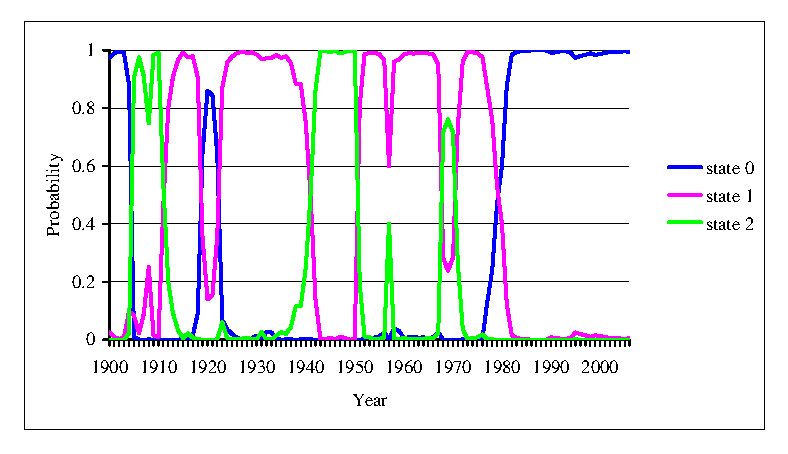
\includegraphics[scale=0.82]{earthquake2.eps}
\caption[Earthquake data: State profiles computed by the
 forward-backward algorithm]
{\textit{Earthquake data: State profiles computed by the
 forward-backward algorithm.}}
\label{fig:earthquakes_smoothed}
%\end{center}
\end{figure}

Since $\log J$ is an
upper bound on $H(S_t| \BSX=\bsx)$, the scale of these entropy profiles is in theory
$\left[ 0,\log3\right] $. However the scale of the entropy profiles is
rather $\left[ 0,\log2\right]$, since in practice at most two states
can explain a given observation equally well; see 
Figure~\ref{fig:eartquakes_mutual}.

In Figure~\ref{fig:eartquakes_mutual}, the mutual 
information $I(S_{t-1};S_t|\mathbf{X}=\mathbf{x})$
between $S_{t-1}$ and $S_t$, given $\mathbf{X}=\mathbf{x}$
is represented, that is, the difference between the marginal and the
conditional entropy at each time $t$:
\[
I(S_{t-1};S_t|\mathbf{X}=\mathbf{x}) =H( S_t%
|\mathbf{X}=\mathbf{x}) -H(S_t|S_{t-1},\mathbf{X}%
=\mathbf{x}).
\]
This mutual information is highly variable as a function of $t$
and the dates where this mutual information is high tend to be
aggregated (between 1912 and 1913, 1920 and 1922, 1939 and 1941, 1969
and 1970, 1978 and 1981 where $I(S_{t-1};S_t|
 \allowbreak \mathbf{X}=\mathbf{x})>0.12$); see
Figure~\ref{fig:eartquakes_mutual}. In these segments $[t,t']$ of high mutual
information, the canonical measure of state uncertainty 
$H(S_t^{t'}|\mathbf{X}=\mathbf{x})$ is far less than
suggested by the marginal entropies, and consequently by the posterior
state probabilities. 

\begin{figure}[!htb]
%\begin{center}
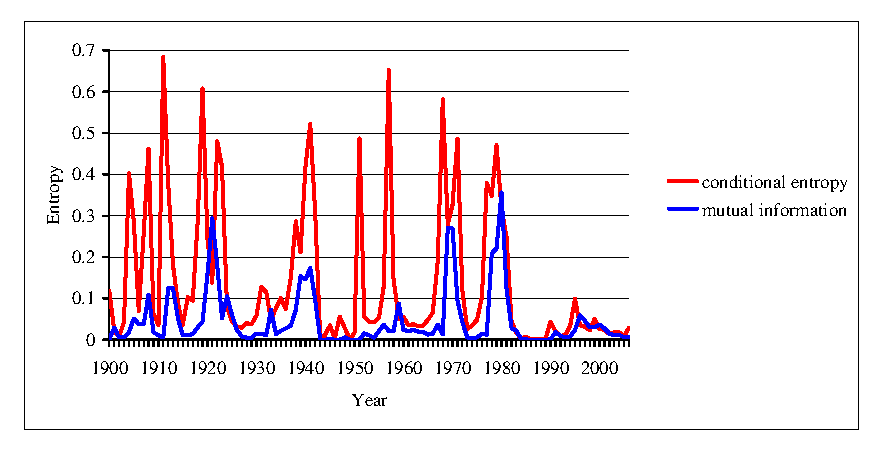
\includegraphics[scale=0.82]{earthquake3.eps}
\caption[Earthquake data: Profiles of conditional entropies and of
mutual information]
{\textit{Earthquake data: Profiles of conditional entropies and of
mutual information.}}
\label{fig:eartquakes_mutual}
%\end{center}
\end{figure}

\subsection{Analysis of the structure of Aleppo pines}
\label{subsec:app_hmt}
The aim of this study was to build a model of the architectural
development of Aleppo pines. 
Its has been shown previously that HMC and HMT models can be used to
analyse the architectural development of fruit and forest trees over
several years on the basis of retrospective measurements of annual
shoot characteristics; see Durand {\it et al.}
(2005\nocite{durand2005}) and Gu\'edon {\it et al.}
(2007a\nocite{guedon2007a}). In HMT models, variables $X_u$ are 
observed along a given tree $\Tree$ with vertex set $\MU$ used 
as index for the observed process $\BSX=(X_u)_{u \in \MU}$.

This type of model enables typical  
successions of annual shoots to be identified
and characterised within tree structures. These successions generally extend
from long polycyclic highly branched annual shoots in proximal
positions to sterile or reproductive short monocyclic unbranched
annual shoots in distal positions in the Aleppo pine case. Regarding
biology, one strength of this approach is the capability to infer
complex dynamical information on the basis of retrospective measurements.

The data set is composed of seven branches
of Aleppo pines ({\it{Pinus Halepensis}} Mill., {\it{Pinaceae}}) planted
in the south of France (Clapiers, H\'erault). The branches came from
seven different 
individuals aged between 35 to 40 years. They were 
described at the scale of annual shoot, defined as the segment of stem
established within a year. A given year of growth can be divided 
into three periods of potential growth, referred to as {\it{(growth) cycles}}. 
For a given annual shoot, if growth occurred during the first cycle only, 
it is said to be {\it{monocyclic}}. Otherwise, growth occurred during 
the first cycle and at least one more cycle, and the annual shoot 
is said to be {\it{polycyclic}}. Moreover, a given annual shoot may 
or not bear sexual organs: female cones, male cones, or no cone at all.
In the latter case, the annual shoot it is said to be {\it{sterile}}.
Five variables were recorded for each annual shoot: length (in cm), number of 
branches per tier, number of growth cycles beyond the first one and
presence or absence of female cones and of male cones. 
% The number of growth cycles beyond the first one
% corresponds to the third recorded variable. 
On these seven branches, a total of 836 annual shoots was measured.

\paragraph{Competing models}
%\label{subsubsec:models}
An HMT model was estimated on the basis of the seven branches, to identify
categories of annual shoots with comparable values for the variables,
and to characterise the succession of the categories within the branches.
The set of parameters $\theta$ (including the initial and transition 
probabilities and the emission distribution parameters) was estimated 
using the EM algorithm for HMT models -- see 
Crouse {\it{et al.}}(1998\nocite{crouse1998}). 
The branches were considered as mutually independent random realizations
of a same HMT model (the trees have 
same parameter set but different structures.)
Except for the length variable, the emission
distributions were multinomial distributions $\MM(1; p_1, \ldots,
p_N)$, where $N$ denotes the number of possible values for this 
variable. Four families of parametric discrete distributions 
were considered for the emission distributions associated with 
the length variable: uniform, Poisson, binomial and 
negative binomial families of distributions, 
each with an additional shift parameter. 
The family associated with the maximum likelihood of the parameters
was selected (in our case, negative binomial distributions for each state).
The five variables were assumed independent given the state.
The number of HMT states could not be deduced {\it{a priori}} from
biological arguments, so it had to be determined using model selection
criteria. We resorted to ICL-BIC (McLachlan \& Peel, 2000, chap. 6) to
select this number. ICL-BIC is defined by
\[
{\mbox{ICL-BIC}}(J) = 2 \log P_{\hat{\theta}_J}(\bsx)
- 2 H(\BSS|\BSX=\bsx) - d_J \log(n)
\]
where $n$ is the number of vertices in $\BSX$, 
$P_{\theta}(\bsx)$ the likelihood of parameter $\theta$,
${\hat \theta}_J$ the estimated parameters 
for a $J$-state HMT model, 
$d_J$ the number of independent model parameters, and the
entropy $H(\BSS|\BSX=\bsx)$ 
is computed as shown in Section \ref{sec:profiles_hmt}.
ICL-BIC incorporates the aim of obtaining non-ambiguous state
restoration in model selection.

The maximal number of possible states was set to 10, and a 6-state model
was selected (with an ICL-BIC value of -10,704) followed by 5-state and
4-state models (with respective values of BIC -10,742 and -10,764). 

\paragraph{Entropy profiles in the 6-state HMT model}
%\label{subsubsec:application-length}
The estimated transition matrix of the 6-state HMT model is
\[
{\hat P} = 
\left[
\begin{array}{llllll}
0.17    & 0.14   & 0.44  & 0.01  & 0  & 0.24 \\
0    & 0.18   & 0.18  & 0  & 0  & 0.64 \\
0    & 0.07   & 0.03  & 0.90  & 0  & 0 \\      
0    & 0.07   & 0.03  & 0  & 0.76  & 0.14 \\
0    & 0   & 0  & 0  & 0  & 1 \\
0    & 0   & 0  & 0  & 0  & 1
\end{array}
\right].
\]
The Markov tree is initialised in state 0 with probability 1. It can be seen
from ${\hat P}$ that the Markov tree has transient state 0, transient
class \{1, 2, 3\}, transient state 4 and absorbing state 5. Hence,
only states 1, 2 and 3 can be visited more than once along a path
within a tree.
State transitions and an interpretation of the hidden states are
provided in Figure~\ref{fig:hmt_diagram}.
In particular, the states are ordered by decreasing length, except 
state 5, which corresponds to slightly longer shoots than state 4.

To quantify the separability between consecutive states $i$ and $j$ (i.e. such that $p_{ij}>0$), we computed distances between the corresponding discrete emission distributions for each observed variable in the form $1- \sum_y \min \{ b_i(y),b_j(y) \}$. This distance, which is one minus the overlap between the two emission distributions, is between 0 (full overlap, i.e. identical distributions) and 1 (no overlap). For quantitative variables (shoot length in our case), this distance is also the sup-norm distance between the two emission distributions (i.e. the maximum absolute difference between the cumulative distribution functions) in the case of non-crossing cumulative distribution functions

\[
1-\underset{y}{\sum} \min \{ b_i(y),b_j(y) \} = \underset{y}{\sup} \left| \overset{y}{\underset{x=0}{\sum}}b_j(x)-\overset{y}{\underset{x=0}{\sum}}b_i(x) \right|.
\]

In our case of multivariate observations, we only give the highest
distance among the five distances computed for each pair of states and
for each variable;
see Table \ref{tab:sup-norm_distances}. This highest distance is
assumed to reflect the separability between consecutive states.
It appears that the 6 states are well separated, except pairs $(2,3)$
and $(3,5)$. However, unbranched, monocyclic, sterile 
shoots can be in any of the states 0, 2, 3 and 5 (respectively with
probability 0.001, 0.261, 0.367 and 0.371). This characteristic of the
model will be shown to be the source of state uncertainty for such
shoots.

\begin{table}[!htb]
\begin{center}
\begin{tabular}[]{cccccccccc}
\hline
States & $0 \to 1$ & $0 \to 2$ & $0 \to 3$ & $1 \to 2$ & $2 \to 3$ &
$3 \to 1$ & $3 \to 4$ & $3 \to 5$ & $4 \to 5$ \\
\hline
sup-norm & 0.85 &  0.80  &  0.89 & 0.78 & 0.20 & 0.98 &  0.99 & 0.48 &
0.97\\
distance & & & & & & & & & \\
\hline 
most & & & & & & & & & \\
separated & br. & fem. & fem. & br. & br. &
br. & male & len. & male \\
variable & & & & & & & & & \\
\hline
\end{tabular}


\caption[Sup-norm distances between emission distributions]
{\textit{Distances between emission distributions for pairs
    of successive states, for the variable that achieves the maximal
    distance among the five variables (br. -- branching;
    fem. -- female cones; len. -- length; male -- male cones.)}}
\label{tab:sup-norm_distances}
\end{center}
\end{table}

\begin{figure}[!htb]
\begin{center}
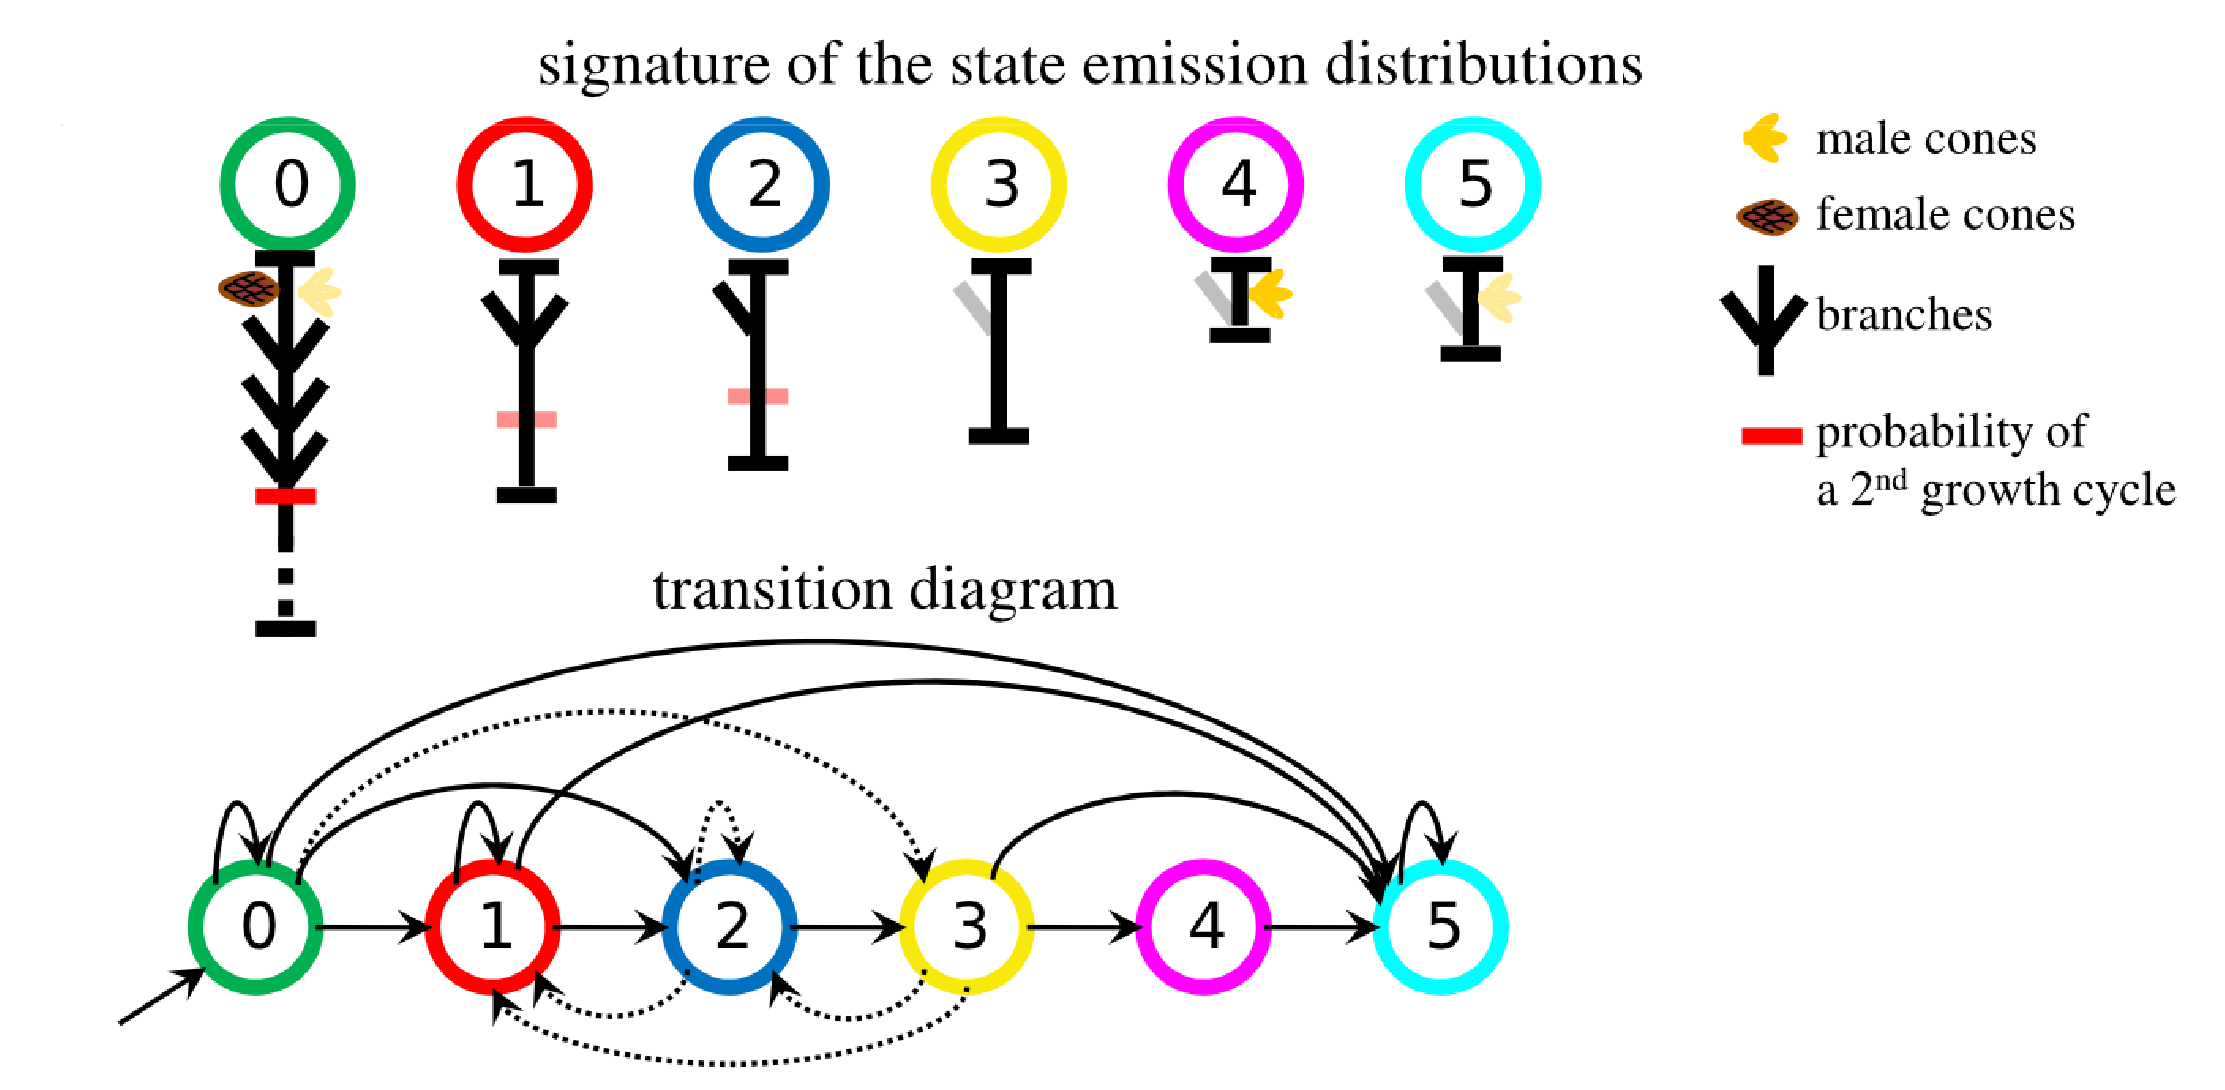
\includegraphics[width=12cm]{hmt6L}
\caption[6-state HMT model: transition diagram and emission distributions]
{\textit{6-state HMT model: transition diagram and symbolic
 representation of the state 
 signatures (conditional mean values of the variables given the states,
 depicted by typical shoots). 
The separation between growth cycle is represented by 
a horizontal red segment, which intensity is proportional to the
probability of occurrence of a second growth cycle.
Dotted arrows correspond to transitions
 with associated probability $< 0.1$. Mean shoot lengths given each state are
 proportional to segment lengths, except for state 0 (which mean length
 is slightly more than twice the mean length for 
state 1).}}
\label{fig:hmt_diagram}
\end{center}
\end{figure}

To analyse how state ambiguity due to unbranched, monocyclic, sterile
shoots affects state restoration, entropy profiles were computed for
each individual (namely, each branch). Firstly, the annual shoots were
represented using a colourmap, which is a mapping between colours and the
values of conditional entropies $H(S_u|S_{\rho(u)}, \BSX=\bsx)$ 
(see Figure~\ref{fig:B3_conditional_entropy_viterbi}a) ). Vertices with lowest
conditional entropy are represented in blue, whereas those with highest
conditional entropy are in red. 

\begin{figure}[!htb]
\begin{center}
\begin{tabular}{cc}
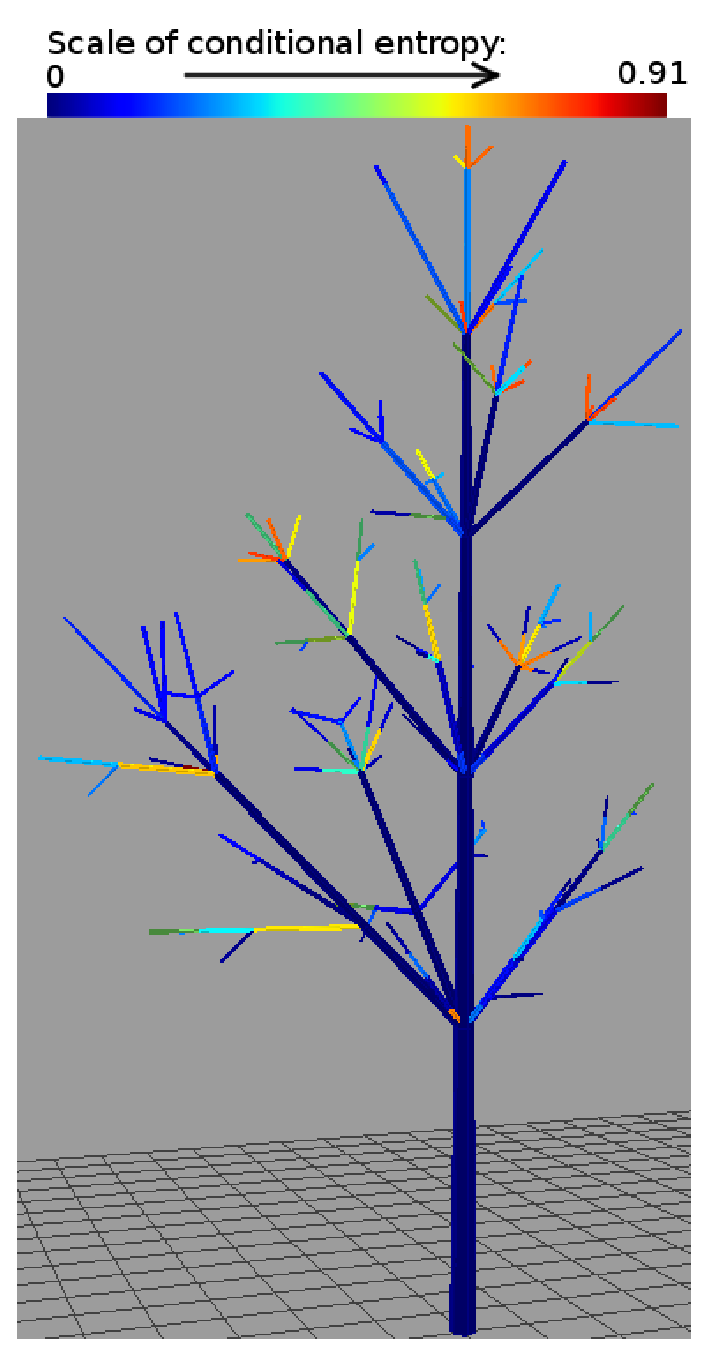
\includegraphics[width=6cm]{B3_downward_entropy6l_color_legend}
 & 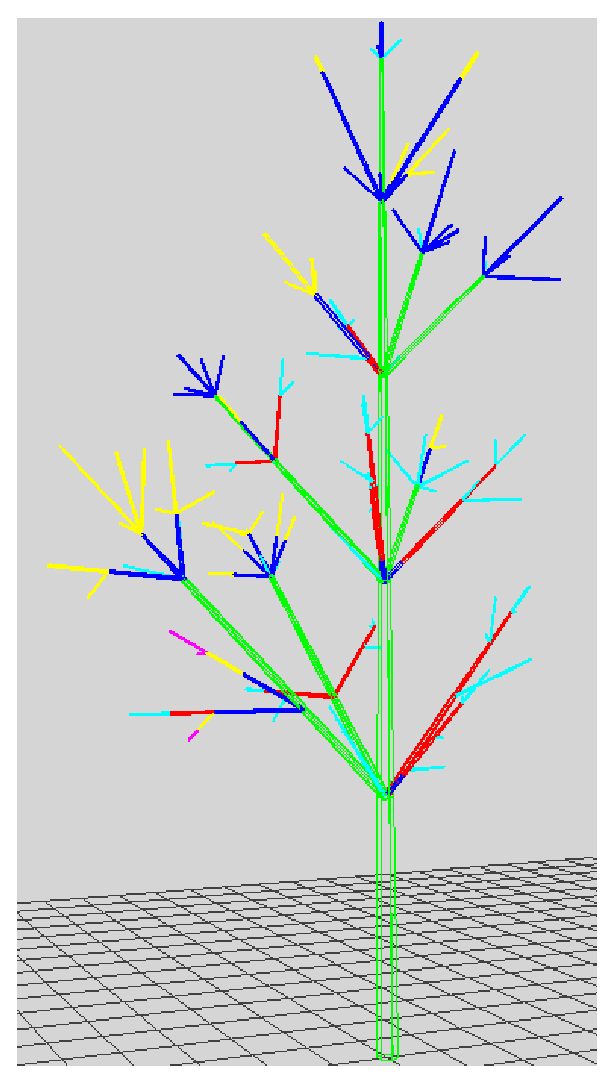
\includegraphics[width=6cm]{B3_viterbi6l} \\
a) & b)
\end{tabular}
\caption[Conditional entropy and state tree restoration]
{\textit{Conditional entropy and state tree restoration for a given
 branch. a) Conditional entropy $H(S_u | S_{\rho(u)}, \BSX = \bsx)$ 
 using a colourmap. Blue  corresponds to lowest entropy and red to
 highest entropy. b) State tree restoration. The correspondence  
 between states and colors is as follows: state 0 - green ; state 1 -
 red ; state 2 - blue ; state 3 - yellow ; state 4 - magenta ; state 5 -
 cyan.}}
\label{fig:B3_conditional_entropy_viterbi}
\end{center}
\end{figure}

The most likely state tree for each individual was computed using the
Viterbi algorithm for HMT models (Durand {\it{et al.}},
2004\nocite{durand2004}). This state tree is represented in Figure 
\ref{fig:B3_conditional_entropy_viterbi}b. This representation shows
where the states are located within the tree; for example state 0 is
located on the main axis (main stem) and at the basis of lateral
axis. Moreover, in conjunction with Figure
\ref{fig:B3_conditional_entropy_viterbi}a, it highlights some states
for which the restoration step is not much ambiguous (in our example,
states 0, 3, 4, and 1 to a least extent). Thus, these states with low 
conditional entropy correspond to vertices with the highest number 
of branches, female or male cones. On the contrary, the vertices with 
highest conditional entropy are mostly unbranched, monocyclic and sterile, 
and are located at peripheral parts of the plant. 

A two-step analysis was performed to identify locations
characterised by particularly high state
uncertainty. The profile of conditional entropies in Figure
\ref{fig:B3_conditional_entropy_viterbi}a was used in a first step to
select zones of vertices with high conditional entropies.
In a second step, local alternatives to the Viterbi restoration were
identified, using the so-called {\it{upward-downward Viterbi
profiles}} as a complement to the entropy profiles.
They rely on the following quantities
\[
\max_{(\bss_v)_{v \neq u}} P((S_v = s_v)_{v \neq u}, S_u=j | \BSX=\bsx),
\]
for each state $j$ and each vertex $u$ of the tree. Their computation is
based on upward and downward dynamic programming recursions, similar to
that of Brushe {\it{et al.}} (1998\nocite{brushe1998}), and are not
detailed in this paper. 
They were used by Gu\'edon (2007b\nocite{guedon2007b}) as
diagnostic tools for localization of state uncertainty in the context of
hidden {\mbox{(semi-)}} Markov chains. This analysis leads to detailed
understanding of the roles of the model and the
observed variables to yield especially high or low state
uncertainty, since both cases can be
informative. 
In application of this methodology, two paths (extracted from
two distinct individuals) were chosen for the contrasted situations
they yielded. The detailed analysis of a path containing successive
monocyclic, sterile shoots is provided hereafter. The analysis of a path
containing a female shoot is given in Appendix \ref{app:pine}.

A path essentially composed by monocyclic, sterile shoots is
considered within the fourth individual (for which
$H(\BSS|\BSX=\bsx) = 47.5$).
The path contains 5 vertices, referred to as 
$\{0, \ldots, 4\}$. 
Shoots 0 and 1 are long and highly branched, and thus are in state
0 with probability $\approx 1$ (also, shoot 0 is bicyclic).  
Shoots 2 to 4 are monocyclic and sterile. Shoots 2 and 3 bear one
branch, and can be in states 1 or 2 essentially. Shoot 4 is unbranched
and from the Viterbi profile in Figure~\ref{fig:B3-6l-963v}b), it can
be in states 2, 3 or 5. 
This is summarised by the entropy profiles in Figure~\ref{fig:B3-6l-963v}a).

This conditional entropy profile can be further interpreted, with
contrasted interpretations according to whether mutual information
(represented in Figure~\ref{fig:B3-6l-963v}c)~) is positive or null,
in cases where marginal entropy remains positive. 
On the one hand, $I(S_1;S_2 | \BSX= \bsx) = 0$. This
results from state $S_1$ being known. Thus, conditioning by $S_1$ does
not provide further information on its children state $S_2$. 
On the other hand, $I(S_3;S_4 | \BSX= \bsx) = 0.2$.  Uncertainty 
associated with the posterior distribution of $S_4$ is high, since 
$H(S_4|\BSX= \bsx) = 0.67$. 
However, knowledge of its parent state $S_3$ would reduce the 
uncertainty on $S_4$: if $S_3=1$ then $S_4=5$; if $S_3=2$ then $S_4=2$
(or less likely, $S_4=3$) and if $S_3=3$ then $S_4=5$ (or less likely,
$S_4=2$). 

Using Proposition \ref{prop:subtree_entropy} in
Appendix~\ref{app:subtree}, the contribution  
of the vertices of the considered path $\MP$ to the global state tree
entropy can be computed as:
\begin{eqnarray}
H(S_0 |\BSX = \bsx)
+ \sum_{u \in \MP \atop u \neq 0 } H(S_u | S_{\rho(u)}, \BSX = \bsx),
\end{eqnarray}
and is equal to 1.41 in the above example (that is, 0.28 per vertex
on average). The global state tree entropy for this individual is 0.24
per vertex, against 0.20 per vertex in the whole dataset.
This is explained by the lack of information brought by the observed
variables (several successive sterile monocyclic shoots, which can be
in states 1, 2, 3 or 5). 

The contribution of $\MP$ to the global state tree entropy
corresponds to the sum of the heights of every point 
of the profile of conditional entropies in Figure~\ref{fig:B3-6l-963v}a). 

Note that the representation of state uncertainty using
profiles of posterior state probabilities induces a perception of global
uncertainty on the states along $\MP$ equivalent to that provided by
marginal entropy profile in Figure~\ref{fig:B3-6l-963v}a). The mean
marginal state entropy for this individual is 0.37 per vertex, which
strongly overestimates the mean state tree entropy.

\begin{figure}[!htb]
\begin{center}
\begin{tabular}{cc}
%\hspace{-2cm}
%\includegraphics[width=7cm]{B3-6l-963v-entropy-upwd} &
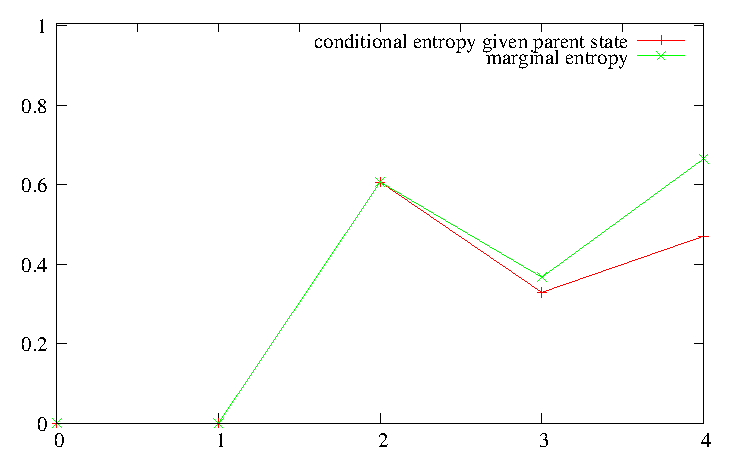
\includegraphics[width=7cm]{B3-6l-963v-entropy-dwd} &
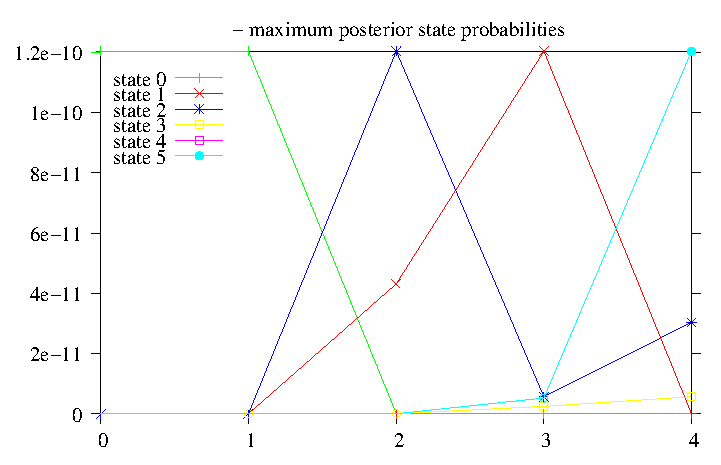
\includegraphics[width=7cm]{B3-6l-963v-viterbi-ud} \\
a) & b) 
\end{tabular}
\begin{tabular}{c}
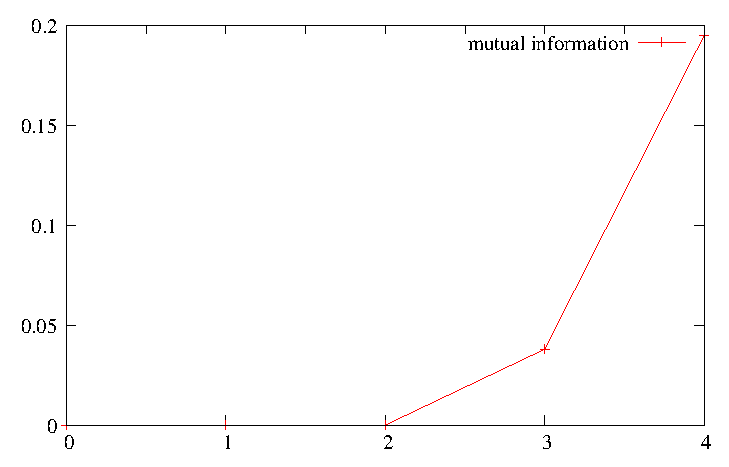
\includegraphics[width=6.5cm]{B3-6l-963v-entropy-dwd-mutual} \\
c)
% vertex 963
\end{tabular}
\end{center}
\caption[Entropy profiles: path containing mainly sterile monocyclic
 shoots]
{\textit{Entropy profiles along a path containing mainly sterile
 monocyclic shoots. 
a) Profiles of conditional and of marginal entropies.
b) State tree restoration with the Viterbi upward-downward
 algorithm. c) Mutual information between a state and its parent
 state.}}
\label{fig:B3-6l-963v}
\end{figure}

This example shows that detailed insight can be brought by joint use of
entropy profiles and the Viterbi algorithm with its variants. The
assignment of states to vertices performed by the model 
is a global operation; however, the local role of the observed data and the
neighbouring states can be understood precisely, by combination 
of the Viterbi algorithm and conditional entropy profiles.

\paragraph{Comparison between marginal and conditional entropy profiles}
As discussed in Section \ref{sec:profiles_hmt}, the following inequality
is satisfied, regarding entropy profiles:
\begin{align*}
G(\Tree) = 
\sum_{u \in \Tree} H(S_u | S_{\rho(u)}, \BSX = \bsx) 
\leq M(\Tree) =  \sum_{u \in \Tree} H(S_u | \BSX = \bsx),
\end{align*}
that is, the global state tree entropy is bounded from above by the
sum of marginal entropies.

To assess the overestimation of state uncertainty induced by using the
profiles based on the marginal entropies $H(S_u | \BSX = \bsx)$
instead of $H(S_u | S_{\rho(u)}, \BSX = \bsx)$, these quantities were 
computed for each tree in the dataset. The ratios
$(M(\Tree)-G(\Tree))/G(\Tree)$ are given in Table 
\ref{tab:parent_children_profiles}.
\begin{table}[!htb]
\begin{center}
\begin{tabular}[]{cccccccc}
\hline
Tree $\Tree$ & 1 & 2 & 3 & 4 & 5 & 6 & 7 \\
            %${\dps{\underline{C(\Tree)-G(\Tree)}}}$ & ${\underline{M(\Tree)-G(\Tree)}}$ 
            %\\ % & $\sqrt{(Var(N_u))}$ \\
number & & & & & & & \\ % & \\
%\hline
\hline
${\dps{\frac{M(\Tree)-G(\Tree)}{G(\Tree)}}}$
& 69.1 \% &  78.0 \%  &  76.4 \% &  56.0 \% & 85.2 \%  &  73.5 \%  &  85.1 \% \\

\hline
\end{tabular}


\caption[Comparison between sums of entropies]
{\textit{Relative distance $(M(\Tree)-G(\Tree))/G(\Tree)$ 
 between sum of marginal entropies $M(\Tree)$ and global state tree
 entropy $G(\Tree)$.}}
\label{tab:parent_children_profiles}
\end{center}
\end{table}

It can be seen from Table \ref{tab:parent_children_profiles} that
$M(\Tree)$ is a poor approximation of the global state tree 
entropy. As a consequence, the posterior state probability 
profiles cannot be used to quantify local contributions
to global state uncertainty.

\section{Concluding remarks}
\label{sec:conclusion}

This article proposes a new methodology to assess state uncertainty in
GHM models. It has been shown that global state entropy can be
decomposed additively along the graph structure. Each element of
the decomposition can be interpreted in terms of local state
uncertainty, corresponding to conditional entropy. This makes it
relevant to draw profiles of conditional entropies, indexed by the graph
vertices. In the particular case of HMC and HMT models, we provided
efficient algorithms to compute these profiles.

Used jointly with the Viterbi algorithm and its variants, these profiles
allow deeper understanding of the local roles of the model parameters, the
neighbouring states and the observed data, concerning state uncertainty. This
leads to a much more efficient approach than the plain Viterbi algorithm
and the posterior state probability profiles to analyse alternative 
state restorations, which may involve zones of connected vertices. 
Such situations are characterised by high mutual information
between connected vertices. Moreover, we showed using examples
that the posterior state probability profiles 
introduce confusion between 
(i) local state uncertainty due to overlap of emission distributions
for different states and (ii) mere propagation of uncertainty 
from past to future states. Contrary to conditional entropy 
profiles, they suggest strong local contributions to global state 
uncertainty in zones where such uncertainty is in fact far more limited.

In Durand \& Gu\'edon (2012\nocite{durand2012}), algorithms similar to
those presented in Section \ref{sec:profiles_hmc} have been proposed
for computing profiles of entropies conditional on the next
state in the HMC model case. This provides the other possible decomposition of the global state
sequence entropy:
\[
H(\BSS|\BSX=\bsx)
=\sum\limits_{t=0}^{T-2}
H(S_t|S_{t+1},\BSX=\bsx) +H(S_{T-1}|\BSX=\bsx).
\]

The interpretation of the profile of entropies conditional on the next
state $\left\{H(S_t|S_{t+1},\BSX=\bsx)\right\}_{t=0,\ldots, T-1}$ is far less obvious than that of the profile of entropies conditional on the previous state $\left\{H(S_t|S_{t-1},\BSX=\bsx)\right\}_{t=0,\ldots,T-1} $
except in the case of reversible processes. In the same way, profiles of
entropies conditional on the children states $\left\{H(S_u | \BSS_{c(u)}, \BSX = \bsx)\right\}_{u \in \MU}$ were obtained in the HMT model case. Contrarily to the profile of
entropies conditional on the parent state $\left\{H(S_u | S_{\rho(u)}, \BSX = \bsx)\right\}_{u \in \MU} $,
the profile of entropies conditional on the children states 
does not constitute a decomposition of global state tree 
entropy and we proved (Durand \& Gu\'edon, 2012\nocite{durand2012}) that
\[
H(\BSS | \BSX= \bsx) \leq \sum_u H(S_{u} | \BSS_{c(u)}, \BSX = \bsx).
\]

Equivalent algorithms remain to be derived for trees with conditional
dependency between children states given parent state (in particular,
for trees oriented from the leaf vertices toward the root), and in the
case of the DAG structures mentioned in Section \ref{subsec:graphical_hmm}.

Stronger connexions can be hypothesised between entropy and the
so-called generalised Viterbi algorithm, which enumerates the $L$ state
sequences or trees $\bss$ with highest probabilities. In particular, the notion
of typical set allows the cardinality of a subset of possible values of
$\bss$ with given minimal probability to be bounded by some functions of
the entropy (Cover and Thomas, 2006\nocite{cover2006}). This could lead to a
bound on the value of $L$ to be used in the generalised Viterbi algorithm.

In the perspective of model selection, entropy computation may also appear
as a valuable tool. If irrelevant states are added to a GHM model,
global state entropy is expected to 
increase. This principle can be extended to adding irrelevant variables
(that is, variables that are independent from the states or conditionally
independent from the states given other variables). This results from
perturbations in the state conditional distribution induced by estimation
from a finite sample.
This intuitive statement explains why several model selection criteria
based on a compromise between log-likelihood and state entropy were 
proposed. Among these is the Normalised 
Entropy Criterion introduced by Celeux  \& Soromenho
(1996\nocite{celeux1996}) in independent mixture models, and
ICL-BIC criterion introduced by McLachlan \& Peel
(2000\nocite{mclachlan2000}, chap. 6). Their generalization to GHM
models is rather straightforward. By favouring models with small state
entropy and high log-likelihood, these criteria aim at selecting models
such as the uncertainty of the state values is low, whilst achieving
good fit to the data. 

\newpage

\appendix
\section*{Appendix.}
\setcounter{proposition}{0}
\renewcommand{\theproposition}{\Alph{section}\arabic{proposition}}
%\label{app:theorem}
% Partial state tree entropies can be obtained for two families of
% subtrees $\left\{H(\BBSS_u | \BSX = \bsx)\right\}_{u \in \MU}$  and
% $\left\{H(\BBSS_{0 \backslash u} | \BSX = \bsx)\right\}_{u \in \MU, u
%   \neq 0}$, using the conditional entropy profiles 
% $\left\{H(S_u| S_{\rho(u)}, \BSX=\bsx)\right\}_{u \in \MU}$ and
% the marginal entropies
% \[
%  H(S_{u} | \BSX = \bsx) = -\sum_j \xi_u(j) \log \xi_u(j).
% \] 
% Computation of 
% these partial state tree entropies is obtained from the following
% lemma: 
\section{Computation of the global entropy of state subtrees in hidden Markov tree models}
\label{app:subtree}

 \begin{proposition}
 Let $\MV$ be a subtree of $\Tree$ with root vertex $r$. 
 Then for any possible value
 $\bbss_\MV$ of $\BBSS_\MV$ and for any $\bsx$,
 \[
 P(\BBSS_\MV = \bbss_\MV | \BSX=\bsx) = P(S_r=s_r| \BSX=\bsx) 
 \prod_{u \in \MV \atop u \neq r} P(S_u=s_u|S_{\rho(u)}=s_{\rho(u)},
 \BSX=\bsx)
 \]
 and
 \[
 H(\BBSS_\MV | \BSX=\bsx) = H(S_r | \BSX=\bsx) 
 + \sum_{u \in \MV \atop u \neq r} H(S_u|S_{\rho(u)}, \BSX=\bsx).
 \]
 \label{prop:subtree_entropy}
 \end{proposition}
 \begin{proof}
 This is proved by induction on the vertices in $\MV$. The induction
 step is as follows: let $\ell$ be a leaf vertex of $\MV$. Then for any
 possible value $\bbss_\MV$ of $\BBSS_\MV$,
 \begin{align*}
 & P(\BBSS_\MV = \bbss_\MV | \BSX=\bsx)  \\
 & = P(S_{\ell}=s_{\ell}|\BBSS_{\MV \backslash \{\ell\}} = \bbss_{\MV
   \backslash \{\ell\}}, \BSX=\bsx)  
 P(\BBSS_{\MV \backslash \{\ell\}} = \bbss_{\MV
   \backslash \{\ell\}} | \BSX=\bsx) \\
  & = P(S_{\ell}=s_{\ell}|S_{\rho(\ell)} = s_{\rho(\ell)},
 \BSX=\bsx) 
 P(\BBSS_{\MV \backslash \{\ell\}} = \bbss_{\MV
   \backslash \{\ell\}} | \BSX=\bsx)
 \end{align*}
 since $S_{\ell}$ is conditionally independent from the other vertices
 in $\MV$ given $S_{\rho(\ell)}$ and $\BSX$.

 The induction step is completed by observing that $\MV \backslash
 \{\ell\}$ is a subtree of $\Tree$. 

 The decomposition of the entropy of $\BBSS_\MV$ yielded by the chain rule
 \[
 H(\BBSS_\MV | \BSX=\bsx) = H(S_r | \BSX=\bsx) 
 + \sum_{u \in \MV \atop u \neq r} H(S_u|S_{\rho(u)}, \BSX=\bsx)
 \]
 is proved similarly as Corollary \ref{cor:graph_entropy}.
 $\blacksquare$
 \end{proof}

\section{Direct computation of global state tree entropy in hidden Markov tree models}
%{Proof of propositions}
%\label{app:proof}

% \subsection{Algorithms for computing entropy profiles conditional on the future
% in the case of hidden Markov chain models}
% \label{future entropy profiles}

% Entropy profiles conditional on the future states rely on the following
% decomposition of the entropy of the state sequence, as a sum of
% local entropies where state $S_t$ at time $t$ is conditional on the
% future states:
% \[
% H\left( \BSS|\BSX=\bsx)
% =\sum\limits_{t=0}^{T-2}
% H\left( S_t|S_{t+1},\BSX=\bsx) +H\left(
% S_{T-1}|\BSX=\bsx) .
% \]
% This is a consequence of the reverse state process being a Markov chain,
% given $\BSX=\bsx$.
% % and from application of equation \eqref{eq:conditional_markov_sequence}.

% Computation of partial state sequence entropies
% $H(S_t^{T-1}|\BSX=\bsx)$ for $t=T-1,\ldots,0$ relies on the following
% backward recursion to compute $H(S_{t+1}^{T-1}|S_t=j,X_{t+1}^{T-1}=x_{t+1}^{T-1})$ 
% for $j=0,\ldots,J-1$ and $t=T-1,\ldots,0$. This algorithm
% is initialised at $t=T-1$ and for $j=0,\ldots,J-1$ as follows:
% \begin{align*}
% & 
% H(S_{T-1}|S_{T-2}=j,X_{T-1}=x_{T-1}) \\
% & =-\sum\limits_{k=0}^{J-1} P(S_{T-1}=k|S_{T-2}=j,X_{T-1}=x_{T-1}) \log P(
% S_{T-1}=k|S_{T-2}=j,X_{T-1}=x_{T-1}).
% \end{align*}
% The backward recursion, similar to that of Hernando {\it{et al.}}
% (2005\nocite{hernando2005}) is given, for $t=T-2,\ldots,0$ and for 
% $j=0,\ldots,J-1$, by:
% \begin{align}
% & H(S_{t+1}^{T-1}|S_t=j,X_{t+1}^{T-1}=x_{t+1}^{T-1})
% \nonumber \\
% & = - \sum\limits_{s_{t+1},\ldots,s_{T-1}} 
% P(
% S_{t+1}^{T-1}=s_{t+1}^{T-1}|S_t=j,X_{t+1}^{T-1}=x_{t+1}^{T-1})
% \log P(
% S_{t+1}^{T-1}=s_{t+1}^{T-1}|S_t=j,X_{t+1}^{T-1}=x_{t+1}^{T-1})
% \nonumber \\
% & = - \sum\limits_{s_{t+2},\ldots,s_{T-1}} \sum\limits_{k=0}^{J-1}
% P(S_{t+2}^{T-1}=s_{t+2}^{T-1}|S_{t+1}=k,S_t=j,X_{t+1}^{T-1}=x_{t+1}^{T-1})
% P(S_{t+1}=k | S_t=j,X_{t+1}^{T-1}=x_{t+1}^{T-1})
% \nonumber \\
% & \times \left\{
% \log
% P(S_{t+2}^{T-1}=s_{2+1}^{T-1}|S_{t+1}=k,S_t=j,X_{t+1}^{T-1}=x_{t+1}^{T-1}) +
% \log P(S_{t+1}=k |
% S_t=j,X_{t+1}^{T-1}=x_{t+1}^{T-1})\right\} \nonumber \\
% & = - \sum\limits_{k=0}^{J-1} P(S_{t+1}=k |
% S_t=j,X_{t+1}^{T-1}=x_{t+1}^{T-1}) 
% \sum\limits_{s_{t+2},\ldots,s_{T-1}} 
% P(S_{t+2}^{T-1}=s_{t+2}^{T-1}|S_{t+1}=k,X_{t+2}^{T-1}=x_{t+2}^{T-1})
% \nonumber \\
% & \times \left\{
% \log
% P(S_{t+2}^{T-1}=s_{2+1}^{T-1}|S_{t+1}=k,X_{t+2}^{T-1}=x_{t+2}^{T-1}) +
% \log P(S_{t+1}=k |S_t=j,
% X_{t+1}^{T-1}=x_{t+1}^{T-1})\right\} 
% \nonumber \\
% & =\sum\limits_{k=0}^{J-1} P(S_{t+1}=k|S_t=j,X_{t+1}^{T-1}=x_{t+1}^{T-1}) \left\{
% H(S_{t+2}^{T-1}|S_{t+1}=k,X_{t+2}^{T-1}=x_{t+2}^{T-1})
% \right.
% \nonumber \\
% & \qquad \left. -\log P(S_{t+1}=k|S_t=j,X_{t+1}^{T-1}=x_{t+1}%
% ^{T-1}) \right\},  \label{entropy_backward_recursion}%
% \end{align}
% with
% \begin{align*}
% & P(S_{t+1}=k|S_t=j,X_{t+1}^{T-1}=x_{t+1}^{T-1}) \\
% & =\frac{P(X_{t+1}^{T-1}=x_{t+1}^{T-1},S_{t+1}=k|S_t=j)
% }{P(X_{t+1}^{T-1}=x_{t+1}^{T-1}|S_t=j) }\\
% & =\frac{L_{t+1}( k) p_{jk}/G_{t+1}( k) }{%
% \sum_m
% L_{t+1}( m) p_{jm}/G_{t+1}( m) }.
% \end{align*}
% \noindent Using a similar argument as in
% \eqref{entropy_backward_recursion}, the termination step is given by
% \begin{align*}
% & H(S_0^{T-1}|\BSX=\bsx) \\
% %& = -\sum\limits_{s_0,\ldots,s_{T-1}} 
% %P(S_0^{T-1}=s_0^{T-1}|\BSX=\bsx)
% %\log P(S_0^{T-1}=s_0^{T-1}|\BSX=\bsx) \\
% %& = -\sum\limits_{s_1,\ldots,s_{T-1}} \sum\limits_{j=0}^{J-1}
% %P(S_1^{T-1}=s_1^{T-1}|S_0=j, \BSX=\bsx)
% %P(S_0=j | \BSX=\bsx) \\
% %& \times \left\{\log P(S_1^{T-1}=s_1^{T-1}|S_0=j,
% % \BSX=\bsx) + \log 
% %P(S_0=j | \BSX=\bsx)\right\} \\
% & = - \sum\limits_{j=0}^{J-1} P(S_0=j | \BSX=\bsx)
% \left\{ \sum\limits_{s_1,\ldots,s_{T-1}} 
% P(S_1^{T-1}=s_1^{T-1}|S_0=j, X_1^{T-1}=x_1^{T-1})
% \right. \\
% & \left. 
% \vphantom{\sum\limits_{s_1,\ldots,s_{T-1}} 
% P}
% \times \log P(S_1^{T-1}=s_1^{T-1}|S_0=j,
% X_1^{T-1}=x_1^{T-1}) + \log 
% P(S_0=j | \BSX=\bsx)\right\} \\
% & = \sum\limits_{j=0}^{J-1}  L_0(j) \left\{
% H(S_1^{T-1}=s_1^{T-1}|S_0=j, X_1^{T-1}=x_1^{T-1})
% - \log L_0(j) \right\}.
% \end{align*}

% Using similar arguments as in \eqref{partial entropy recursion},
% we have
% \begin{eqnarray}
% H(S_t^{T-1}|\BSX=\bsx)
% =\sum\limits_{j=0}^{J-1}
% L_t( j ) \left\{ 
% H(S_{t+1}^{T-1}|S_t=j,X_{t+1}^{T-1}=x_{t+1}^{T-1}) 
% -\log L_t(j) \right\}.
% \label{eq:cmc_reverse_entropy}
% \end{eqnarray}
% Thus, the profile of partial state sequence entropies 
% $\left\{H(S_t^{T-1}|\BSX=\bsx)\right\}_{t=0,\ldots,T-1}$ 
% can be computed as a byproduct of the
% forward-backward algorithm, where the usual backward recursion
% \eqref{backward recursion} and the backward recursion 
% for conditional entropies \eqref{entropy_backward_recursion} are
% mixed. The conditional entropies 
% are then directly deduced by first-order differencing
% \begin{align*}
% H(S_t|S_{t+1},\BSX=\bsx)  & =H(
% S_t|S_{t+1}^{T-1},\BSX=\bsx) \\
% & =H(S_t^{T-1}|\BSX=\bsx) -H(
% S_{t+1}^{T-1}|\BSX=\bsx).
% \end{align*}
% The profile of conditional entropies $\left\{ H(S_t|S_{t+1}
% ,\BSX=\bsx)\right\}_{t=0,\ldots,T-1}$ can also be
% computed directly, as
% \begin{align*}
%  H(S_t|S_{t+1},\BSX=\bsx) % \\
%  =-\sum\limits_{j,k}
% P(S_t=j,S_{t+1}=k|\BSX=\bsx) \log P(
% S_t=j|S_{t+1}=k,\BSX=\bsx)
% \end{align*}
% with%
% \begin{align*}
% P(S_t=j|S_{t+1}=k,\BSX=\bsx)  & =P(
% S_t=j|S_{t+1}=k,X_0^t=x_0^t) \\
% & =p_{jk}F_t( j) /G_{t+1}( k) \, {\mbox{ and }}\\
% P(S_t=j,S_{t+1}=k|\BSX=\bsx)  & =L_{t+1}(
% k) p_{jk}F_t( j) /G_{t+1}( k) .
% \end{align*}

% The latter quantities are directly extracted during the forward
% (\ref{forward recursion}) and backward recursions (\ref{backward recursion})
% of the forward-backward algorithm. The conditional entropy is bounded from
% above by the marginal entropy (Cover \& Thomas (2006\nocite{cover2006}),
% chap. 2):
% \[
% H(S_t|S_{t+1},\BSX=\bsx) \leq H(
% S_t|\BSX=\bsx) .
% \]

%\subsection{Direct computation of conditional entropy of children state
%  subtrees given each state in hidden Markov tree models}
\label{app:hmt_hernando}

\noindent Direct computation of global state tree entropy is based on
recursive computation of the entropies of children state
    subtrees given each state. 
This recursion relies on conditional independence properties between
hidden and observed variables in HMT models, and particularly the
following relations: 
for any internal, non-root vertex $u$ and for $j = 1,\ldots,J$,
\begin{eqnarray}
{\lefteqn{P(\BBSS_{c(u)} = \bbss_{c(u)} | S_u=j, \BBSS_{0 \backslash u} = \bbss_{0
 \backslash u}, \BSX=\bsx)}} \nonumber \\
& \hspace{5cm} = &  
P(\BBSS_{c(u)} = \bbss_{c(u)} | S_u=j, S_{\rho(u)} = s_{\rho(u)} ,
\BSX=\bsx)  \nonumber \\
& \hspace{5cm} = &  P(\BBSS_{c(u)} = \bbss_{c(u)} | S_u=j, \BSX=\bsx) \nonumber \\
& \hspace{5cm} =& \prod\limits_{v \in c(u)} 
P(\BBSS_v = \bbss_v | S_u=j, \BSX=\bsx) \nonumber \\ 
& \hspace{5cm} =& \prod\limits_{v \in c(u)} 
P(\BBSS_v = \bbss_v | S_u=j, \BBSX_v=\bbsx_v) \label{eq:hmt_cond_ind_prod} \\
& \hspace{5cm} =&  
P(\BBSS_{c(u)} = \bbss_{c(u)} | S_u=j, \BBSX_u=\bbsx_u), % \\
\label{eq:hmt_cond_ind_nd}
\end{eqnarray}
\begin{eqnarray*}
P(\BBSS_u = \bbss_u | \BBSS_{0 \backslash u} = \bbss_{0 \backslash u}, \BSX=\bsx)
& = & P(\BBSS_u = \bbss_u | S_{\rho(u)} = s_{\rho(u)} , \BSX=\bsx) \\
& = &  P(\BBSS_u = \bbss_u | S_{\rho(u)} = s_{\rho(u)}, \BBSX_u=\bbsx_u). % \\
\end{eqnarray*}

Entropies $H(\BBSS_{c(u)} | S_{u}=j, \BBSX_u=\bbsx_u)$
can be computed for any $u \in \MU, u \neq 0$ and
for $j=0,\ldots,J-1$, by an upward algorithm initialised at the leaf
vertices $u$ by 
\[
H(\BBSS_{c(u)}|S_{u}=j,\BBSX_u=\bbsx_u) = 0.
\]

%Since $\BBSS_{c(u)}$ and $\BBSX_{0 \backslash u}$ are conditionally
% independent given $S_u$ and $\BBSX_u$, 
As a consequence from \eqref{eq:hmt_cond_ind_nd}, we have for any state $j$,
$H(\BBSS_{c(u)}|S_{u}=j,\BBSX_u=\bbsx_u) 
= H(\BBSS_{c(u)}|S_{u}=j,\BSX=\bsx)$. Thus, it is deduced from
\eqref{eq:hmt_cond_ind_prod} that
\begin{align}
H(\BBSS_{c(u)}|S_{u}=j,\BBSX_u=\bbsx_u) 
= & H(\BBSS_{c(u)}|S_{u}=j,\BBSX_{c(u)}=\bbsx_{c(u)}) \nonumber \\
= & \sum_{v \in c(u)}H(\BBSS_{v}|S_{u}=j,\BBSX_v=\bbsx_v).
\label{eq:hmt_cond_ind_ch}
\end{align}
% which is similar to the backward recursion
% \eqref{entropy_backward_recursion} in time-reversed HMC models (see
% Appendix \ref{future entropy profiles}).
 
\noindent Moreover, for any $v \in c(u)$ with $c(v) \neq \emptyset$ and
for $j=0,\ldots,J-1$,
\begin{align}
& H(\BBSS_{v}|S_{u}=j,\BBSX_u=\bbsx_u) \nonumber \\
& = -\sum_{\bbss_{c(v)}, s_v} P(\BBSS_{c(v)}=\bss_{c(v)}, S_v=s_v |
 S_u=j,\BBSX_u=\bbsx_u) \nonumber \\
& \qquad \times \log P(\BBSS_{c(v)}=\bss_{c(v)}, S_v=s_v |
 S_u=j,\BBSX_u=\bbsx_u) \nonumber \\
& = -\sum_{\bss_{c(v)}} \sum\limits_{k=0}^{J-1} P(\BBSS_{c(v)}=\bss_{c(v)} | 
S_v = k, S_u=j, \BBSX_u=\bbsx_u) 
P(S_v = k | S_u=j, \BBSX_u=\bbsx_u) \nonumber \\
& \qquad \times \{
\log P(\BBSS_{c(v)}=\bss_{c(v)} | S_v = k, S_u=j, \BBSX_u=\bbsx_u) 
+ \log P(S_v = k | S_u=j, \BBSX_u=\bbsx_u) \} \nonumber \\
& = -\sum\limits_{k=0}^{J-1} P(S_v = k | S_u=j, \BBSX_v=\bbsx_v) \left\{
\sum_{\bss_{c(v)}} 
P(\BBSS_{c(v)}=\bss_{c(v)} | S_v = k, \BBSX_v=\bbsx_v) \right. \nonumber \\
& \quad \times \left.
\vphantom{\sum_s P\left(s\right)}
\log P(\BBSS_{c(v)}=\bss_{c(v)} | S_v = k, \BBSX_v=\bbsx_v) 
+ \log P(S_v = k | S_u=j, \BBSX_v=\bbsx_v) \right\} \nonumber \\
& = \sum\limits_{k=0}^{J-1} P(S_v = k | S_u=j, \BBSX_v=\bbsx_v) \left\{
H(\BBSS_{c(v)} | S_v = k, \BBSX_v=\bbsx_v) \right. \nonumber \\
& \qquad \left.
\vphantom{P\left(s\right)}
- \log P(S_v = k | S_u=j, \BBSX_v=\bbsx_v) \right\}.
\label{eq:hernando_tree}
\end{align}
Thus, the recursion of
the upward algorithm is given by 
\begin{align}
& H(\BBSS_{c(u)}|S_{u}=j,\BBSX_u=\bbsx_u) 
\label{eq:upwd_state_cond_rec} \\
& =  \sum_{v \in c(u)} \left\{\sum_{s_v} 
P(S_v=s_v | S_u=j, \BBSX_v=\bbsx_v) \left[ 
H(\BBSS_{c(v)}|S_v=s_v, \BBSX_v=\bbsx_v) \right.\right. \nonumber \\
& \quad \left.\left. - \log P(S_v=s_v | S_u=j, \BBSX_v=\bbsx_v)
\right]
\vphantom{+\left\{\sum_{s_v} \right\}}
\right\}, \nonumber 
\end{align}
where $P(S_v=k | S_u=j, \BBSX_v=\bbsx_v) = 
P(S_v=k | S_u=j, \BSX=\bsx)$ is given by equation
\eqref{eq:predict_upwd}. 

The termination step is obtained by similar arguments as equation
\eqref{eq:hmt_cond_ind_ch}:
\begin{align*}
H(\BSS | \BSX = \bsx) = &
H(\BBSS_{c(0)} | S_0, \BSX = \bsx)
+ H(S_0 | \BSX = \bsx) \\
= & \sum\limits_{j=0}^{J-1} \beta_{0}\left(  j\right)  \left\{  H\left(  \BBSS_{c\left(  0\right)
}|S_{0}=j,\BSX = \bsx\right)  -\log\beta_{0}\left(
j\right)  \right\}  .
\end{align*}
% If each vertex has a single child, HMT and HMC models coincide, and
% equation \eqref{eq:upwd_state_cond_rec} appears as a generalization of
% \eqref{eq:cmc_reverse_entropy} for the computation of conditional
% entropies in time-reversed HMCs -- see Appendix \ref{future entropy profiles}.

% By conditional independence of $\BBSS_{c(u)}$ and 
% $\BBSX_{0 \backslash u}$ given $S_u$ and $\BBSX_u$, 
% $H(\BBSS_{c(u)} | S_u=j, \BSX = \bsx) = 
% H(\BBSS_{c(u)} | S_u=j, \BBSX_u = \bbsx_u)$ for any state $j$ and vertex
% $u$.
% Thus, 
Using similar arguments as in \eqref{eq:hernando_tree}, 
the partial state tree entropy $H(\BBSS_u | \BSX = \bsx)$
can be deduced from the conditional entropies 
$H(\BBSS_{c(u)}|S_{u}=j,\BBSX_u=\bbsx_u)$ (with $j=0,\ldots,J-1$) as follows: 
\begin{align}
H(\BBSS_u | \BSX = \bsx) = & H(\BBSS_{c(u)} | S_u, \BSX = \bsx)
+ H(S_u | \BSX = \bsx) \nonumber \\
 = & \sum_j \xi_{u}(j)  \left\{  H\left(\BBSS_{c\left(  u\right)
}|S_{u}=j,\BSX= \bsx \right)  -\log\xi_{u}\left(
j\right)  \right\} \nonumber \\
 = & \sum_j \xi_{u}(j)  \left\{  H\left(\BBSS_{c\left(  u\right)
}|S_{u}=j,\BBSX_u= \bbsx_u \right)  -\log\xi_{u}\left(
j\right)  \right\},
\label{eq:upward_conditional}
\end{align}
where the $\left\{\xi_u(j)\right\}_{j=0,\ldots,J-1}$ are directly extracted from
the downward recursion \eqref{eq:downward}.

The profile of conditional entropies 
$H(S_{u} | S_{\rho(u)}, \BSX = \bsx)$ is deduced from
\begin{align*}
H(\BBSS_{\rho(u)} | \BSX = \bsx) 
= & H(S_{\rho(u)}, \BBSS_{b(u)}, \BBSS_u | \BSX = \bsx) \\
= & H(S_{\rho(u)} | \BSX = \bsx) + H(\BBSS_{b(u)} | S_{\rho(u)}, \BSX = \bsx) 
+ H(\BBSS_{u} |S_{\rho(u)}, \BSX = \bsx),
\end{align*}
where
\begin{align*}
H(\BBSS_{b(u)} | S_{\rho(u)}, \BSX = \bsx) 
= & \sum_{v \in b(u)} H(\BBSS_v | S_{\rho(v)}, \BSX = \bsx) \\
= & \sum_{v \in b(u)} \left\{\sum_j \xi_{\rho(v)}(j) 
H(\BBSS_v | S_{\rho(v)}=j, \BSX = \bsx) \right\},
\end{align*}
and where for any brother vertex $v$ of $u$, 
$H(\BBSS_v | S_{\rho(v)}=j, \BSX = \bsx)$ is given by
\eqref{eq:hernando_tree}. 
Since 
\begin{align*}
H(\BBSS_{v} | S_{\rho(v)}, \BSX = \bsx) 
= \sum_j H(\BBSS_{v} | S_{\rho(v)}=j, \BSX = \bsx) \xi_{\rho(v)}(j)
\end{align*}
and since
\begin{align}
H(\BBSS_u |  S_{\rho(u)}, \BSX = \bsx) 
= & H(S_u |  S_{\rho(u)}, \BSX = \bsx) + H(\BBSS_c(u) | S_u, \BSX = \bsx)
\nonumber \\
= & H(S_u |  S_{\rho(u)}, \BSX = \bsx) + 
\sum_j \xi_u(j) H(\BBSS_{c(u)} | S_u=j, \BSX = \bsx),
\label{eq:conditional_entropy_variant}
\end{align}
$H(S_{u} | S_{\rho(u)}, \BSX = \bsx)$ is directly extracted from the
partial state entropies $H(\BBSS_{c(u)} | S_u=j, \BSX = \bsx)$ and 
$H(\BBSS_{\rho(u)} | \BSX = \bsx)$ and from the marginal entropy
$H(S_{\rho(u)} | \BSX = \bsx)$.

% Moreover, since 
% \begin{align*}
% H(\BBSS_{0 \backslash u} | \BSX = \bsx)
% = & H(\BBSS_{0} | \BSX = \bsx) -  H(\BBSS_{u} | S_{0 \backslash u}, 
% \BSX = \bsx) \\
% = & H(\BBSS_{0} | \BSX = \bsx) -  H(\BBSS_{u} | S_{\rho(u)}, 
% \BSX = \bsx) 
% \end{align*}
% and since
% \begin{align*}
% H(\BBSS_{u} | S_{\rho(u)}, \BSX = \bsx) 
% = H(\BBSS_{c(u)} | S_u, \BSX = \bsx) +  H(S_{u} | S_{\rho(u)}, 
% \BSX = \bsx),
% \end{align*}
% the partial state tree entropy 
% $H(\BBSS_{0 \backslash u} | \BSX = \bsx)$
% can also be deduced from the conditional entropies 
% $\left\{H(\BBSS_{c(u)}|S_{u}=j,\BBSX_u=\bbsx_u)\right\}_{j=0,\ldots,J-1}$ using 
% \begin{align}
% & H(\BBSS_{0 \backslash u} | \BSX = \bsx) \label{eq:ud_entropy} \\
% & =  H(\BBSS_{0} | \BSX = \bsx) 
% - \sum_j \xi_u(j) H(\BBSS_{c(u)}|S_{u}=j,\BBSX_u=\bbsx_u)
% -  H(S_{u} | S_{\rho(u)}, \BSX = \bsx).
% \nonumber
% \end{align}
% % but the computation of $H(S_{u} | S_{\rho(u)}, \BSX = \bsx)$
% % using \eqref{eq:child_parent_entropy} is still necessary.

In summary, the partial subtrees entropies 
$\left\{H(\BBSS_{c(u)}|S_{u}=j,\BBSX_u=\bbsx_u)\right\}_{u \in \MU;}$
${}_{j=0,\ldots,J-1}$ are firstly computed using \eqref{eq:upwd_state_cond_rec}.
The partial state tree entropies 
$\left\{H(\BBSS_u | \BSX = \right.\allowbreak \left.\bsx )\right\}_{u
  \in \MU}$ and then the profile of conditional entropies 
$\left\{H(S_{u} | S_{\rho(u)}, \BSX = \bsx)\right\}_{u \in \MU}$ are
deduced from these entropies and the posterior state probabilities, using
\eqref{eq:upward_conditional} and
\eqref{eq:conditional_entropy_variant}. 
% Computation of partial state tree entropies  
% $\left\{H(\BBSS_{0 \backslash u} | \BSX = \bsx)\right\}_{u \in \MU}$
% relies on \eqref{eq:ud_entropy}. 
The time complexity of the algorithm is in $\MO(J^2n)$.

% \subsection{Entropy profiles conditional on the children states for
%   hidden Markov tree models}
% \label{app:hmt_children_profiles}
% A proof of Proposition \ref{prop:child_entropy} is given, in the case of
% binary trees for the sake of simplicity. 
% \begin{proof}
% Let $lc\left(  u\right)  $ and $rc\left(  u\right)  $ denote the two
% children of vertex $u$. Applying the chain rule on the children of the
% root vertex, we can write
% \begin{align*}
% H\left(  \BSS|\BSX=\bsx\right)   &
% =H\left(  S_{0}|\BBSS_{c\left(  0\right)  },\BSX=\bsx\right)  
% +H\left(  S_{lc\left(  0\right)  }|\BBSS_{c\left(  lc\left(  0\right)
%  \right)  },\BBSS_{rc\left(  0\right) 
% },\BSX=\bsx\right)  \\
% & \quad +  H\left(  S_{rc\left(  0\right)  }|\BBSS_{c\left(  lc\left(
% 0\right)  \right)  },\BBSS_{c\left(  rc\left(  0\right)  \right)
% },\BSX=\bsx\right)  +H\left(  \BBSS_{c\left(
% lc\left(  0\right)  \right)  },\BBSS_{c\left(  rc\left(  0\right)
% \right)  }|\BSX=\bsx\right)  .
% \end{align*}


% This decomposition is indeed not unique and we can choose to extract the
% conditional entropy corresponding to $rc\left(  0\right)  $ before the
% conditional entropy corresponding to $lc\left(  0\right)  $. Applying
% the property that deconditioning augments entropy (Cover \& Thomas,
%  2006\nocite{cover2006}, chap. 2)
% \begin{align*}
% H\left(  S_{lc\left(  0\right)  }|\BBSS_{c\left(  lc\left(  0\right)
% \right)  },\BBSS_{rc\left(  0\right)  },\BSX=\bsx\right)   &  \leq H\left(  S_{lc\left(  0\right)  }|
% \BBSS_{c\left(  lc\left(  0\right)  \right)  },\BSX=\bsx\right)  ,\\
% H\left(  S_{rc\left(  0\right)  }|\BBSS_{c\left(  lc\left(  0\right)
% \right)  },\BBSS_{c\left(  rc\left(  0\right)  \right)  },\BSX=\bsx \right)   &  \leq H\left(  S_{rc\left(  0\right)
% }|\BBSS_{c\left(  rc\left(  0\right)  \right)  },\BSX
% =\bsx\right)  ,
% \end{align*}
% we obtain
% \begin{align*}
% H\left(  \BSS|\BSX=\bsx\right)   &  \leq
% H\left(  S_{0}|\BBSS_{c\left(  0\right)  },\BSX=\bsx\right)  
% +H\left(  S_{lc\left(  0\right)  }|\BBSS_{c\left(  lc\left(  0\right)
%  \right)  },\BSX=\bsx\right)  \\
% & \quad + H\left(  S_{rc\left(  0\right)  }|\BBSS_{c\left(  rc\left(
% 0\right)  \right)  },\BSX=\bsx\right)  +H\left(
% \BBSS_{c\left(  lc\left(  0\right)  \right)  },\BBSS_{c\left(
% rc\left(  0\right)  \right)  }|\BSX=\bsx\right)  .
% \end{align*}
% Applying the same decomposition recursively from the root to
% the leaves and upper bounding on each internal vertex completes the
% proof by induction.
% \end{proof}

\section{Application of HMT model to Aleppo pines: path containing
  female shoots}
\label{app:pine}
A path containing a female shoot is considered. This path
corresponds to the main axis of the third individual (for which
$H(\BSS|\BSX=\bsx) = 29.6$). The path contains
6 vertices, referred to as $\{0, \ldots, 5\}$. The female shoot is at 
vertex 2, and vertex 3 is a bicyclic shoot. Shoots 4 and 5 are
unbranched, monocyclic, sterile shoots. 

The contribution of the vertices of the considered path $\MP$ to the
global state tree is equal to 0.48 (that is, 0.08 per vertex
on average). The global state tree entropy for this individual is 0.21
per vertex, against 0.20 per vertex in the whole dataset.
The mean marginal state entropy for this individual is 0.37 per
vertex, which strongly overestimates the mean state tree entropy.

Since a female shoot necessarily is in state 0, $H(S_2 | \BSX = \bsx)=0$
(no uncertainty). The states of shoots 0 and 1 can be deduced from $S_2$
using the transition matrix ${\hat P}$, thus their marginal entropy is
null. Since shoot 3 is bicyclic, it is in state 0 with a very
high probability ($H(S_3 | \BSX = \bsx) \approx 0$). 
Uncertainty remains concerning the states of shoots 4 and 5, which thus
have high marginal entropies. However, $S_5$ can be deduced from $S_4$
using ${\hat P}$ and inversely, which results into high mutual information
between $S_4$ and $S_5$ given $\BSX = \bsx$.
This is illustrated by conditional and marginal entropy profiles in
Figure~\ref{fig:B2-6l-772v}.  
\begin{figure}[!htb]
\begin{center}
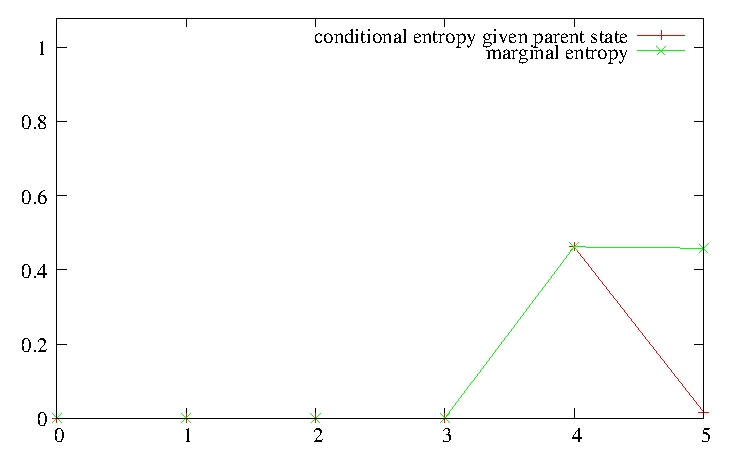
\includegraphics[width=7cm]{B2-6l-772v-entropy-dwd}
\end{center}
\caption[Entropy profiles: path containing a female shoot]
{\textit{Path containing a female shoot: Profiles of conditional and
    of marginal entropies.}} 
\label{fig:B2-6l-772v}
\end{figure}


\begin{acknowledgements}
%If you'd like to thank anyone, place your comments here
%and remove the percent signs.
The authors are indebted to Yves Caraglio for useful comments on modelling
the Aleppo pines dataset and for providing this dataset.
\end{acknowledgements}

% BibTeX users please use one of
%\bibliographystyle{spbasic}      % basic style, author-year citations
% uncomment line below
%\bibliographystyle{spmpsci}      % mathematics and physical sciences
%\bibliographystyle{spphys}       % APS-like style for physics
%\bibliographystyle{jabbrv_acm}

 % name your BibTeX data base
% uncomment line below
% \bibliography{shorttitles,bibliography}

% Non-BibTeX users please use
% \begin{thebibliography}{}
%
% and use \bibitem to create references. Consult the Instructions
% for authors for reference list style.
%
% \bibitem{RefJ}
% Format for Journal Reference
% Author, Article title, Journal, Volume, page numbers (year)
% Format for books
% \bibitem{RefB}
% Author, Book title, page numbers. Publisher, place (year)
% etc
% \end{thebibliography}
\ifx\undefined\allcaps\def\allcaps#1{#1}\fi
\begin{thebibliography}{10}
\providecommand{\url}[1]{{#1}}
\providecommand{\urlprefix}{URL }
\expandafter\ifx\csname urlstyle\endcsname\relax
  \providecommand{\doi}[1]{DOI~\discretionary{}{}{}#1}\else
  \providecommand{\doi}{DOI~\discretionary{}{}{}\begingroup
  \urlstyle{rm}\Url}\fi

% \bibitem{boucheron2007}
% Boucheron, S., Gassiat, E.: An information-theoretic perspective on order
%   estimation, pp. 565--602.
% \newblock O. Capp\'e, E. Moulines and T. Ryd\'en, Springer, New York (2007)

\bibitem{brushe1998}
Brushe, G., Mahony, R., Moore, J.: A {S}oft {O}utput {H}ybrid {A}lgorithm for
  {ML/MAP} {S}equence {E}stimation.
\newblock \allcaps{IEEE} Trans. Inf. Theory \textbf{44}(7), 3129--3134 (1998)

\bibitem{lecadre1998}
Cadre, J.P.L., Tremois, O.: Bearing-{O}nly {T}racking for {M}aneuvering
  {S}ources.
\newblock \allcaps{IEEE} Trans. Aerosp. Electron. Syst. \textbf{34}(1),
  179--193 (1998)

\bibitem{cappe2005}
Capp\'{e}, O., Moulines, E., Ryd\'{e}n, T.: Inference in {H}idden {M}arkov
  {M}odels.
\newblock Springer Series in Statistics. New York: Springer (2005)

% \bibitem{celeux2008}
% Celeux, G., Durand, {\relax{J.\mbox{-}B}}.: {S}electing {H}idden {M}arkov
%   {M}odel {S}tate {N}umber with {C}ross-{V}alidated {L}ikelihood.
% \newblock Comput. Stat. \textbf{23}, 541--564 (2008)

\bibitem{celeux1996}
Celeux, G., Soromenho, G.: An entropy criterion for assessing the number of
  clusters in a mixture model.
\newblock J. Classif. \textbf{13}(2), 195--212 (1996)

\bibitem{cover2006}
Cover, T., Thomas, J.: Elements of Information Theory, 2nd edition.
\newblock Hoboken, NJ: Wiley (2006)

\bibitem{crouse1998}
Crouse, M., Nowak, R., Baraniuk, R.: Wavelet-{B}ased {S}tatistical {S}ignal
  {P}rocessing {U}sing {H}idden {M}arkov {M}odels.
\newblock \allcaps{IEEE} Trans. Signal Process. \textbf{46}(4), 886--902 (1998)

\bibitem{devijver1985}
Devijver, P.A.: Baum's forward-backward {A}lgorithm {R}evisited.
\newblock Pattern Recognit. Lett. \textbf{3}, 369--373 (1985)

\bibitem{durand2013}
Durand, {\relax{J.\mbox{-}B}}., Girard, S., Ciriza, V., Donini, L.:
  Optimization of power consumption and device availability based on point
  process modelling of the request sequence.
\newblock Appl. Stat. \textbf{62}(2), 151--162  (2013)

\bibitem{durand2004}
Durand, {\relax{J.\mbox{-}B}}., Gon\c{c}alv\`{e}s, P., Gu\'{e}don, Y.:
  Computational methods for hidden {M}arkov tree models -- an application to
  wavelet trees.
\newblock \allcaps{IEEE} Trans. Signal Process. \textbf{52}(9), 2551--2560
  (2004)

\bibitem{durand2005}
Durand, {\relax{J.\mbox{-}B}}., Gu\'{e}don, Y., Caraglio, Y., Costes,
E.:
Analysis of the Plant Architecture via Tree-structured Statistical
Models: the Hidden Markov Tree Models.
\newblock New Phytol. \textbf{166}(3), 813--825
  (2005)

\bibitem{durand2012}
Durand, {\relax{J.\mbox{-}B}}., Gu\'edon, Y.:
   Localizing the {L}atent {S}tructure {C}anonical {U}ncertainty: {E}ntropy
   {P}rofiles for {H}idden {M}arkov {M}odels.
\newblock Available: \url{hal.inria.fr/hal-00675223/en}, Inria
technical report
  (2012) 

\bibitem{ephraim2002}
Ephraim, Y., Merhav, N.: Hidden {M}arkov processes.
\newblock \allcaps{IEEE} Trans. Inf. Theory \textbf{48}, 1518--1569 (2002)

\bibitem{guedon2007a}
Gu\'{e}don, Y., Caraglio, Y., Heuret, P., Lebarbier, E., Meredieu, C.:
Analyzing growth components in trees.
\newblock J. Theor. Biol. \textbf{248}(3), 418--447 (2007a)

\bibitem{guedon2007b}
Gu\'{e}don, Y.: Exploring the state sequence space for hidden {M}arkov and
  semi-{M}arkov chains.
\newblock Comput. Stat. Data An. \textbf{51}(5), 2379--2409 (2007b)

\bibitem{guedon2013}
Gu\'{e}don, Y.: Segmentation uncertainty in multiple change-point models.
\newblock Stat. Comput., in press  (2013)

\bibitem{hernando2005}
Hernando, D., Crespi, V., Cybenko, G.: Efficient computation of the hidden
  {M}arkov model entropy for a given observation sequence.
\newblock \allcaps{IEEE} Trans. Inf. Theory \textbf{51}(7), 2681--2685 (2005)

\bibitem{lauritzen1996}
Lauritzen, S.: Graphical {M}odels.
\newblock Clarendon Press, Oxford, United Kingdom (1996)

\bibitem{mclachlan2000}
McLachlan, G., Peel, D.: Finite {M}ixture {M}odels.
\newblock Wiley Series in Probability and Statistics. John Wiley and Sons
  (2000)

\bibitem{zucchini2009}
Zucchini, W., MacDonald, I.: Hidden {M}arkov {M}odels for {T}ime {Series}:
  \textit{{A}n {I}ntroduction {U}sing {R}}.
\newblock Chapman \& Hall/CRC: Boca Raton FL (2009)

\end{thebibliography}
\end{document}
% end of file template.tex
